% !TeX program = xelatex
% 第十九届全国大学生结构设计竞赛理论方案正式提交版
\documentclass[UTF8,a4paper,12pt,fontset=none]{ctexart}

\usepackage{geometry}
\usepackage{graphicx}
\usepackage{fontspec}
\geometry{left=2.55cm,right=2.55cm,top=2.55cm,bottom=2.55cm,headsep=0.45cm}
\usepackage{amsmath,amssymb,bm}
\usepackage{booktabs,longtable,tabularx,array,multirow}
\usepackage{enumitem}
\usepackage{indentfirst}
\usepackage{float}
\usepackage{caption,subcaption}
\usepackage{xcolor}
\usepackage{tikz,pgfplots}
\pgfplotsset{compat=1.18}
\usetikzlibrary{arrows.meta,calc,positioning,patterns,decorations.pathreplacing,shapes.geometric,fit}
\usepackage{fancyhdr}
\usepackage{hyperref}
\usepackage{titlesec}
\usepackage{tocloft}
\usepackage{etoolbox}

% 模板字体设置：正文中文宋体小四，英文 Times New Roman 风格；标题楷体加粗
\setmainfont{Times New Roman}
\setsansfont{Arial}
\setmonofont{Consolas}
\setCJKmainfont[AutoFakeBold=2.5]{SimSun}
\newCJKfontfamily\songti[AutoFakeBold=2.5]{SimSun}
\newCJKfontfamily\kaishu[AutoFakeBold=2.8]{KaiTi}
\newCJKfontfamily\heiti[AutoFakeBold=2.0]{SimHei}

\hypersetup{colorlinks=true, linkcolor=black, urlcolor=black, citecolor=black}
\captionsetup{font=small,labelsep=quad}
\captionsetup[subfigure]{font=small,justification=centering}
\setlength{\parindent}{2em}
\setlength{\parskip}{0.16em}
\linespread{1.30}
\renewcommand{\arraystretch}{1.18}
\setcounter{tocdepth}{2}
\setlist[enumerate]{leftmargin=2.3em,itemsep=0.15em,topsep=0.25em}
\setlist[itemize]{leftmargin=2.3em,itemsep=0.15em,topsep=0.25em}

% 表格字体比正文小一号
\AtBeginEnvironment{table}{\zihao{5}}
\AtBeginEnvironment{longtable}{\zihao{5}}

% 页眉页脚
\pagestyle{fancy}
\fancyhf{}
\fancyhead[C]{\kaishu 第十九届全国大学生结构设计竞赛理论方案}
\fancyfoot[C]{\thepage}
\renewcommand{\headrulewidth}{0.4pt}
\renewcommand{\footrulewidth}{0pt}
\setlength{\headheight}{15pt}

% 标题格式
\titleformat{\section}{\kaishu\bfseries\zihao{-3}}{\thesection}{1em}{}
\titleformat{\subsection}{\kaishu\bfseries\zihao{4}}{\thesubsection}{1em}{}
\titleformat{\subsubsection}{\kaishu\bfseries\zihao{-4}}{\thesubsubsection}{1em}{}
\titlespacing*{\section}{0pt}{1.2em}{0.65em}
\titlespacing*{\subsection}{0pt}{0.85em}{0.45em}
\titlespacing*{\subsubsection}{0pt}{0.60em}{0.35em}

% 目录名称
\renewcommand{\contentsname}{目录}
\renewcommand{\listfigurename}{图目录}
\renewcommand{\listtablename}{表目录}
\renewcommand{\cfttoctitlefont}{\hfill\heiti\bfseries\zihao{3}}
\renewcommand{\cftaftertoctitle}{\hfill}
\renewcommand{\cftloftitlefont}{\hfill\heiti\bfseries\zihao{3}}
\renewcommand{\cftafterloftitle}{\hfill}
\renewcommand{\cftlottitlefont}{\hfill\heiti\bfseries\zihao{3}}
\renewcommand{\cftafterlottitle}{\hfill}
\setlength{\cftbeforesecskip}{0.30em}
\setlength{\cftbeforefigskip}{0.20em}
\setlength{\cftbeforetabskip}{0.20em}

% 章节编号式公式、图、表编号：1-1、1-2
\numberwithin{equation}{section}
\numberwithin{figure}{section}
\numberwithin{table}{section}
\renewcommand{\theequation}{\thesection-\arabic{equation}}
\renewcommand{\thefigure}{\thesection-\arabic{figure}}
\renewcommand{\thetable}{\thesection-\arabic{table}}

\newcolumntype{Y}{>{\raggedright\arraybackslash}X}
\newcolumntype{C}[1]{>{\centering\arraybackslash}p{#1}}
\newcolumntype{L}[1]{>{\raggedright\arraybackslash}p{#1}}
\newcommand{\mm}{\,\mathrm{mm}}
\newcommand{\g}{\,\mathrm{g}}
\newcommand{\kg}{\,\mathrm{kg}}
\newcommand{\cm}{\,\mathrm{cm}}
\newcommand{\Nunit}{\,\mathrm{N}}
\newcommand{\MPa}{\,\mathrm{MPa}}
\newcommand{\GPa}{\,\mathrm{GPa}}
\newcommand{\mss}{\,\mathrm{m/s^2}}
\newcommand{\placeholder}[3][]{%
\begin{figure}[H]
\centering
\begin{tikzpicture}[x=1cm,y=1cm]
  \draw[densely dashed,line width=0.8pt,gray] (0,0) rectangle (13.0,#2);
  \draw[gray!70] (0.25,0.25) rectangle (12.75,#2-0.25);
\end{tikzpicture}
\caption{#3}
\ifstrempty{#1}{}{\label{#1}}
\end{figure}}

\newcommand{\catalogtitle}[1]{%
  \begin{center}
    {\heiti\bfseries\zihao{4} #1}
  \end{center}
  \vspace{-0.4em}
}

\tikzset{
  beam/.style={line width=1.7pt,draw=black,fill=brown!22},
  hollow/.style={line width=1.2pt,draw=black,fill=brown!16},
  rod/.style={line width=1.0pt,draw=brown!65!black},
  load/.style={-Latex,line width=0.8pt,red!75!black},
  react/.style={-Latex,line width=0.9pt,green!55!black},
  forceblue/.style={-Latex,line width=0.9pt,blue!70!black},
  note/.style={draw=black!45,rounded corners=1mm,fill=white,inner sep=3pt,font=\zihao{5}},
  bluecard/.style={draw=blue!55!black,fill=blue!7,rounded corners=1.8mm,minimum width=3.1cm,minimum height=0.95cm,align=center,font=\zihao{5}},
  greencard/.style={draw=green!45!black,fill=green!8,rounded corners=1.8mm,minimum width=3.1cm,minimum height=0.95cm,align=center,font=\zihao{5}},
  orangecard/.style={draw=orange!65!black,fill=orange!12,rounded corners=1.8mm,minimum width=3.1cm,minimum height=0.95cm,align=center,font=\zihao{5}},
  redcard/.style={draw=red!50!black,fill=red!7,rounded corners=1.8mm,minimum width=3.1cm,minimum height=0.95cm,align=center,font=\zihao{5}},
  flowarrow/.style={-{Latex[length=2.6mm,width=2.0mm]},line width=0.95pt,draw=black!75},
  keymark/.style={draw=red!75!black,line width=1.05pt,rounded corners=1.2mm},
  keyarrow/.style={-{Latex[length=2.4mm,width=1.8mm]},draw=red!75!black,line width=0.95pt},
  softlabel/.style={draw=black!35,fill=white,rounded corners=1.2mm,inner sep=3pt,font=\zihao{5}},
  axisgrid/.style={gray!35,line width=0.35pt}
}

\begin{document}
\songti\zihao{-4}
\pagenumbering{arabic}

%------------------ 封面 ------------------
\thispagestyle{fancy}
\vspace*{0.6cm}
\begin{center}
{\heiti\bfseries\zihao{2} 第十九届全国大学生结构设计竞赛理论方案}\par
\vspace{4.2cm}
{\heiti\bfseries\zihao{2}《勒勒车模型结构设计与制作》}\par
\vfill
{\heiti\bfseries\zihao{3} 第十九届全国大学生结构设计竞赛组织委员会}\par
\vspace{0.8cm}
{\heiti\bfseries\zihao{3} 2026 年 10 月}\par
\end{center}
\newpage

%------------------ 目录、图目录、表目录 ------------------
\thispagestyle{fancy}
\tableofcontents
\newpage
\phantomsection
\addcontentsline{toc}{section}{图目录}
\catalogtitle{图目录}
{\zihao{5}
\begin{longtable}{@{}C{1.8cm}L{8.7cm}C{1.4cm}C{1.4cm}@{}}
\toprule
\textbf{图号} & \textbf{图名} & \textbf{页数} & \textbf{页码} \\
\midrule
\endfirsthead
\toprule
\textbf{图号} & \textbf{图名} & \textbf{页数} & \textbf{页码} \\
\midrule
\endhead
图\ref{fig:logic} & 理论方案编制与实物校核流程 & 1 & \pageref{fig:logic} \\
图\ref{fig:scheme-photos} & 三种候选车架方案原型照片 & 1 & \pageref{fig:scheme-photos} \\
图\ref{fig:scheme-score} & 三种候选方案综合评分对比 & 1 & \pageref{fig:scheme-score} \\
图\ref{fig:overall-model} & 最终采用的空心双主梁勒勒车模型总体示意 & 1 & \pageref{fig:overall-model} \\
图\ref{fig:beam-model} & 单根主梁等效简支梁模型 & 1 & \pageref{fig:beam-model} \\
图\ref{fig:section-compare} & 方形空心截面与等面积实心杆对比 & 1 & \pageref{fig:section-compare} \\
图\ref{fig:thickness-sensitivity} & 主梁壁厚对弯曲应力的影响 & 1 & \pageref{fig:thickness-sensitivity} \\
图\ref{fig:rod-support} & 布袋底面与多道横向小杆共同承托示意 & 1 & \pageref{fig:rod-support} \\
图\ref{fig:crossbar-layout} & 不同横向小杆布置的承托示意 & 1 & \pageref{fig:crossbar-layout} \\
图\ref{fig:wheel-reaction} & 轮轴与车身支承反力示意 & 1 & \pageref{fig:wheel-reaction} \\
图\ref{fig:axle-align} & 轮轴同轴度校正示意 & 1 & \pageref{fig:axle-align} \\
图\ref{fig:joint-peel} & 横杆端部胶接节点优化示意 & 1 & \pageref{fig:joint-peel} \\
图\ref{fig:screw-node} & 四螺丝牵引连接节点示意 & 1 & \pageref{fig:screw-node} \\
图\ref{fig:connection-detail} & 关键连接构造优化示意 & 1 & \pageref{fig:connection-detail} \\
图\ref{fig:slope-force} & 坡道牵引与布袋防滑示意 & 1 & \pageref{fig:slope-force} \\
图\ref{fig:stability} & 弯道抗倾覆与重心投影示意 & 1 & \pageref{fig:stability} \\
图\ref{fig:dynamic-reaction} & 动力放大系数与车轮反力关系 & 1 & \pageref{fig:dynamic-reaction} \\
图\ref{fig:torsion} & 单桥工况下车架抗扭示意 & 1 & \pageref{fig:torsion} \\
图\ref{fig:risk-map} & 典型工况风险分布图 & 1 & \pageref{fig:risk-map} \\
图\ref{fig:bag-efficiency} & 装载袋数对载质比的影响 & 1 & \pageref{fig:bag-efficiency} \\
图\ref{fig:loading-plan} & 40 袋装货平面布置示意 & 1 & \pageref{fig:loading-plan} \\
图\ref{fig:center-control} & 满载码放的重心控制示意 & 1 & \pageref{fig:center-control} \\
图\ref{fig:gantt} & 现场制作时间甘特图 & 1 & \pageref{fig:gantt} \\
图\ref{fig:check-flow} & 制作完成后的校核流程图 & 1 & \pageref{fig:check-flow} \\
图\ref{fig:precheck-card} & 赛前核查卡片示意 & 1 & \pageref{fig:precheck-card} \\
图\ref{fig:field-photos} & 实物模型、加载试验和满载行驶照片 & 1 & \pageref{fig:field-photos} \\
图\ref{fig:summary-route} & 作品设计与优化过程概述 & 1 & \pageref{fig:summary-route} \\
图\ref{fig:work-photo} & 作品照片 & 1 & \pageref{fig:work-photo} \\
\bottomrule
\end{longtable}
}
\newpage
\phantomsection
\addcontentsline{toc}{section}{表目录}
\catalogtitle{表目录}
{\zihao{5}
\begin{longtable}{@{}C{1.8cm}L{8.7cm}C{1.4cm}C{1.4cm}@{}}
\toprule
\textbf{表号} & \textbf{表名} & \textbf{页数} & \textbf{页码} \\
\midrule
\endfirsthead
\toprule
\textbf{表号} & \textbf{表名} & \textbf{页数} & \textbf{页码} \\
\midrule
\endhead
表\ref{tab:rules-response} & 赛题约束与本方案响应 & 1 & \pageref{tab:rules-response} \\
表\ref{tab:modules} & 计算模块划分表 & 1 & \pageref{tab:modules} \\
表\ref{tab:scheme-compare} & 三种方案比选表 & 1 & \pageref{tab:scheme-compare} \\
表\ref{tab:scheme-score} & 三种候选方案加权评分表 & 1 & \pageref{tab:scheme-score} \\
表\ref{tab:body-params} & 车身模块主要计算参数 & 1 & \pageref{tab:body-params} \\
表\ref{tab:thickness-sensitivity} & 主梁壁厚变化对受力性能的影响 & 1 & \pageref{tab:thickness-sensitivity} \\
表\ref{tab:crossbar-layout} & 横向小杆布置方案比较 & 1 & \pageref{tab:crossbar-layout} \\
表\ref{tab:body-summary} & 车身模块关键结果汇总 & 1 & \pageref{tab:body-summary} \\
表\ref{tab:wheel-control} & 轮轴模块控制项目 & 1 & \pageref{tab:wheel-control} \\
表\ref{tab:rolling-resistance} & 滚动阻力系数对行驶阻力的影响 & 1 & \pageref{tab:rolling-resistance} \\
表\ref{tab:joint-summary} & 连接模块计算结果汇总 & 1 & \pageref{tab:joint-summary} \\
表\ref{tab:connection-control} & 关键节点构造控制表 & 1 & \pageref{tab:connection-control} \\
表\ref{tab:dynamic-reaction} & 动力放大系数对单侧车轮反力的影响 & 1 & \pageref{tab:dynamic-reaction} \\
表\ref{tab:condition-envelope} & 典型工况风险等级与控制重点 & 1 & \pageref{tab:condition-envelope} \\
表\ref{tab:case-summary} & 专项工况风险与控制措施 & 1 & \pageref{tab:case-summary} \\
表\ref{tab:mass-sensitivity} & 附加质量对载质比的影响 & 1 & \pageref{tab:mass-sensitivity} \\
表\ref{tab:bag-efficiency} & 不同装载袋数下的载质比比较 & 1 & \pageref{tab:bag-efficiency} \\
表\ref{tab:loading-time} & 40 袋装货顺序与时间分配 & 1 & \pageref{tab:loading-time} \\
表\ref{tab:make-time} & 14 小时制作时间分配 & 1 & \pageref{tab:make-time} \\
表\ref{tab:load-test-plan} & 分级加载试验方案 & 1 & \pageref{tab:load-test-plan} \\
表\ref{tab:tolerance} & 关键尺寸控制表 & 1 & \pageref{tab:tolerance} \\
表\ref{tab:deflection-record} & 满载挠度实测记录表 & 1 & \pageref{tab:deflection-record} \\
表\ref{tab:run-record} & 行驶试验记录表 & 1 & \pageref{tab:run-record} \\
表\ref{tab:risk-list} & 现场风险清单与处理措施 & 1 & \pageref{tab:risk-list} \\
表\ref{tab:work-summary} & 作品主要特点汇总 & 1 & \pageref{tab:work-summary} \\
\bottomrule
\end{longtable}
}
\newpage

\section{赛题分析与设计要求}

\subsection{任务边界}
本计算书对应《勒勒车模型结构设计与制作》赛题。模型由车架、车轮、车轴、轴承以及动力小车连接件组成。车轴、轴承和轴卡由组委会统一提供，车轮只能通过轴承与车轴连接；模型在行驶全过程中，除车轮外，其余部位不得与赛道或障碍物接触。

货物为内装玻璃颗粒布袋，单袋质量约 $500\g$。参赛队可选择 $20\sim40$ 袋。本队采用满载 $40$ 袋策略，目标是在保证通过率的前提下提高载质比。布袋按层叠方式摆放，不采用捆绑、夹紧或粘接等固定方式；靠近动力小车一侧的布袋边缘与动力小车 E 面保持不小于 $20\mm$ 的净距。

\begin{table}[H]
\centering
\caption{赛题约束与本方案响应}
\label{tab:rules-response}
\begin{tabularx}{\linewidth}{cY Y}
\toprule
序号 & 赛题约束 & 本方案响应 \\
\midrule
1 & 布袋数量为 $20\sim40$ 袋，每袋约 $500\g$ & 按 $40$ 袋满载设计，计算有效货物质量 \\
2 & 布袋只能层叠放置，不得捆绑 & 采用承托和浅限位，不写作固定或绑扎 \\
3 & 车轮只能通过轴承与车轴连接 & 车轮、轴承、车轴作为独立行走模块计算 \\
4 & 除车轮外模型不得接触赛道和障碍物 & 进行离地、减速带和单桥专项分析 \\
5 & 理论方案重在科学性、完整性和表达清晰 & 按模块拆分计算，图表与公式按章节编号 \\
\bottomrule
\end{tabularx}
\end{table}

\subsection{设计目标}
设计目标分为承载、通过、轻量和制作四类。承载目标是满载 $40$ 袋时车身主承重体系不发生破坏，挠度不影响布袋稳定；通过目标是通过坡道、弯道、减速带和单桥时不侧翻、不刮碰、不掉袋；轻量目标是减少低效率填充材料，提高运输成本得分；制作目标是在现场规定时间内完成加工、装配和试装。

计算目的：确定满载货物的重力，作为后续车身模块、轮轴模块和连接节点模块的共同输入荷载。

\begin{equation}
  G=N_i m_0 g
\end{equation}

式中，$G$ 为货物总重；$N_i$ 为布袋数量；$m_0$ 为单袋质量；$g$ 为重力加速度。

代入本方案数据：
\begin{equation}
  G=40\times0.5\times9.8=196\Nunit
\end{equation}

\subsection{计算模块划分}
本计算书将结构拆分为四个独立计算模块，并将专项工况单独归类。各模块的边界、输入和输出见表\ref{tab:modules}。

\begin{table}[H]
\centering
\caption{计算模块划分表}
\label{tab:modules}
\begin{tabularx}{\linewidth}{cY Y Y}
\toprule
模块 & 分析对象 & 主要计算内容 & 输出结论 \\
\midrule
车身模块 & 左右方形空心主梁、横向小杆、承托区 & 截面性质、弯曲强度、挠度、横杆分配 & 车身是否能承受满载 \\
轮轴模块 & 车轮、轴承、车轴、轴承座 & 车轮反力、轴承座局部承压、行走阻力 & 行走支承是否可靠 \\
连接模块 & 胶接节点、四螺丝牵引连接板 & 胶缝剪应力、孔边承压、牵引力传递 & 节点是否可靠 \\
专项工况 & 坡道、弯道、减速带、单桥、装货 & 防滑、抗倾覆、冲击放大、抗扭 & 运输过程是否稳定 \\
\bottomrule
\end{tabularx}
\end{table}

\begin{figure}[H]
\centering
\begin{tikzpicture}[x=1cm,y=1cm,every node/.style={font=\zihao{5}},>=Latex]
  \node[bluecard,minimum width=1.75cm,text width=1.45cm] (a) at (0.0,0) {1\\约束\\边界};
  \node[bluecard,minimum width=1.75cm,text width=1.45cm] (b) at (2.05,0) {2\\方案\\原型};
  \node[greencard,minimum width=1.75cm,text width=1.45cm] (c) at (4.10,0) {3\\模块\\计算};
  \node[orangecard,minimum width=1.75cm,text width=1.45cm] (d) at (6.15,0) {4\\工况\\验算};
  \node[orangecard,minimum width=1.75cm,text width=1.45cm] (e) at (8.20,0) {5\\制作\\校核};
  \node[redcard,minimum width=1.75cm,text width=1.45cm] (f) at (10.25,0) {6\\总结\\定稿};
  \foreach \from/\to in {a/b,b/c,c/d,d/e,e/f}{\draw[flowarrow] (\from) -- (\to);}
  \draw[keymark] ($(c.south west)+(-0.05,-0.08)$) rectangle ($(d.north east)+(0.05,0.08)$);
  \node[draw=red!75!black,fill=white,rounded corners=1.2mm,inner sep=3pt,align=center] (k1) at (5.12,1.35) {关键控制点\\强度、挠度、质量};
  \draw[keyarrow] (k1.south) -- ($(c.north)!0.5!(d.north)$);
  \draw[keymark] ($(e.south west)+(-0.05,-0.08)$) rectangle ($(f.north east)+(0.05,0.08)$);
  \node[draw=red!75!black,fill=white,rounded corners=1.2mm,inner sep=3pt,align=center] (k2) at (9.22,-1.25) {实物落实\\尺寸、节点、装货};
  \draw[keyarrow] (k2.north) -- ($(e.south)!0.5!(f.south)$);
\end{tikzpicture}
\caption{理论方案编制与实物校核流程}
\label{fig:logic}
\end{figure}

\newpage
\section{方案构思与原型照片}

\subsection{候选方案原型照片}
选型阶段按“三选一”方式提出三种候选车架方案。比选不仅关注强度是否满足要求，还同步比较重量、荷载效率和制作工艺三个维度。若某一方案虽然质量较轻，但现场制作难度过高、节点误差难以控制，则不作为最终方案。

三种候选方案原型照片如图\ref{fig:scheme-photos}所示。

\begin{figure}[H]
\centering
\begin{subfigure}[t]{0.32\linewidth}
  \centering
  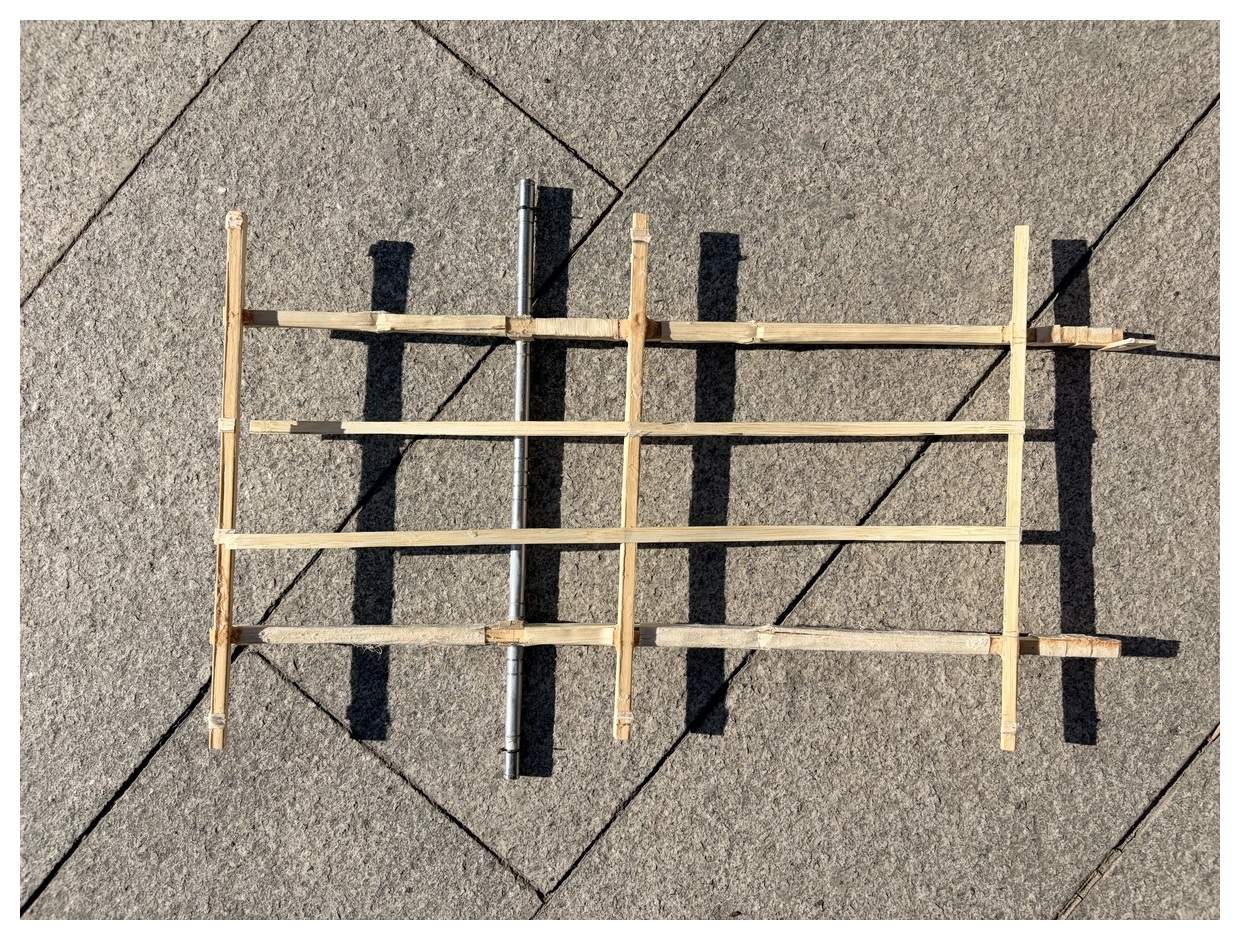
\includegraphics[width=\linewidth]{images/schemeA_photo2.jpg}
  \caption{方案 A：平板承托式}
\end{subfigure}\hfill
\begin{subfigure}[t]{0.32\linewidth}
  \centering
  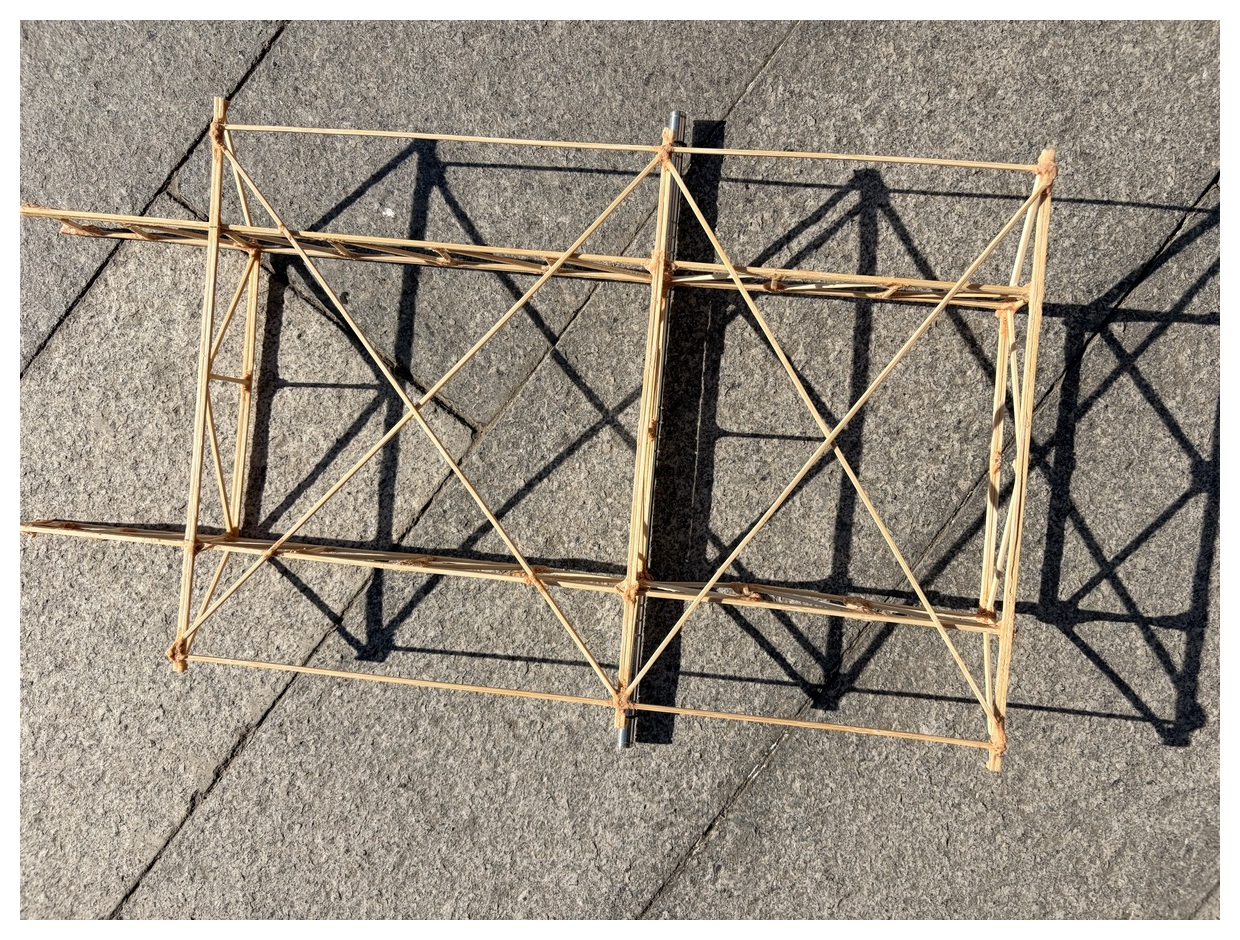
\includegraphics[width=\linewidth]{images/schemeB_photo2.jpg}
  \caption{方案 B：箱型空间桁架式}
\end{subfigure}\hfill
\begin{subfigure}[t]{0.32\linewidth}
  \centering
  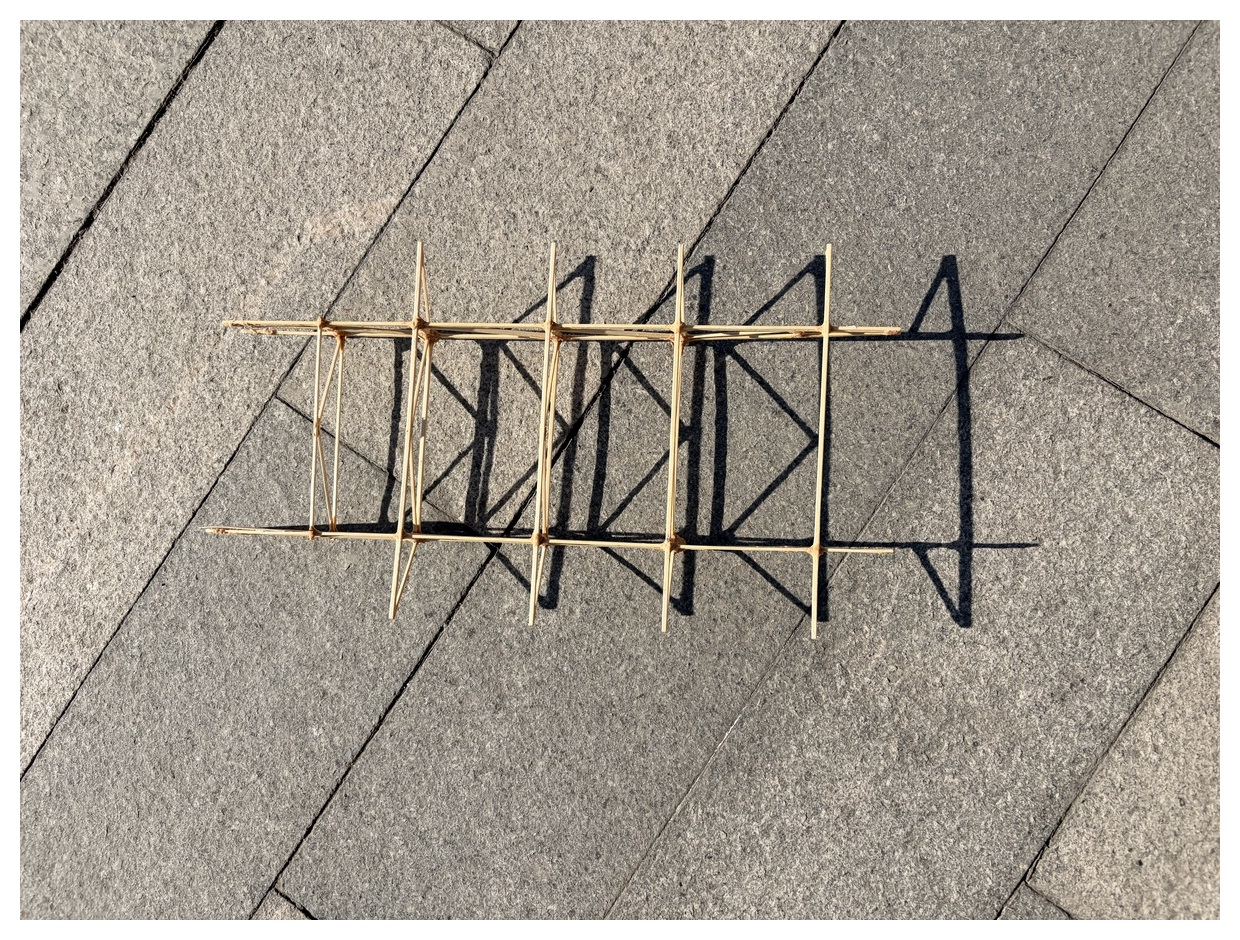
\includegraphics[width=\linewidth]{images/schemeC_photo2.jpg}
  \caption{方案 C：双纵梁格构承托式}
\end{subfigure}
\caption{三种候选车架方案原型照片}
\label{fig:scheme-photos}
\end{figure}

\subsection{三维度比选}
比选维度包括重量、荷载效率和制作工艺。重量主要影响载质比；荷载效率反映单位材料形成抗弯刚度的能力；制作工艺反映现场可实现性和误差控制难度。

\begin{table}[H]
\centering
\caption{三种方案比选表}
\label{tab:scheme-compare}
\begin{tabularx}{\linewidth}{cY c c c Y}
\toprule
方案 & 结构形式 & 重量 & 荷载效率 & 制作工艺 & 结论 \\
\midrule
A & 平板承托式车架 & 偏大 & 中等 & 简单 & 承托面较大、装货直观，但材料利用率偏低，自重较大，淘汰 \\
B & 箱型空间桁架式车架 & 最小 & 较高 & 困难 & 杆件数量多、节点繁杂，现场加工和胶接误差难控制，淘汰 \\
C & 双纵梁格构承托式车架 & 较小 & 高 & 中等 & 在质量、承载与工艺之间综合最优，确定为后续优化基础方案 \\
\bottomrule
\end{tabularx}
\end{table}

方案 A 的主要优点是布袋接触面较大、摆放直观，但纵向构件和横向承托条较多，导致单位承载对应的自重偏大；方案 B 的理论重量最低，结构效率也较高，但需要大量斜杆和精细节点，现场 14 小时内难以稳定保证每个节点的胶接质量；方案 C 兼顾了较好的承托连续性和较少的关键节点，综合表现最佳，因此被选为最终方案的原型基础。

\subsection{定量评分结果}
为进一步降低方案判断的主观性，采用加权评分法对三种候选方案进行定量比较。根据本赛题“轻量、高效、可制作”的要求，取重量、荷载效率和制作工艺的权重分别为 $0.35$、$0.35$ 和 $0.30$。各维度按 $10$ 分制评分，结果见表\ref{tab:scheme-score}。

\begin{table}[H]
\centering
\caption{三种候选方案加权评分表}
\label{tab:scheme-score}
\begin{tabular}{c c c c c}
\toprule
方案 & 重量得分 & 荷载效率得分 & 制作工艺得分 & 加权总分 \\
\midrule
A & 6 & 6 & 9 & 6.90 \\
B & 9 & 8 & 4 & 7.10 \\
C & 8 & 9 & 8 & 8.35 \\
\bottomrule
\end{tabular}
\end{table}

\begin{figure}[H]
\centering
\begin{tikzpicture}[x=1cm,y=0.95cm,every node/.style={font=\small}]
  \foreach \x in {0,1,...,10}{\draw[axisgrid] (\x,0.2)--(\x,3.8);} 
  \draw[-Latex,line width=0.9pt] (0,0.2)--(10.5,0.2) node[right]{综合评分/分};
  \foreach \x/\lab in {0/0,2/2,4/4,6/6,8/8,10/10}{\node[below] at (\x,0.15){\lab};}
  \node[left] at (-0.1,0.95){A 方案};
  \node[left] at (-0.1,2.00){B 方案};
  \node[left] at (-0.1,3.05){C 方案};
  \filldraw[fill=blue!18,draw=blue!65!black,rounded corners=1mm] (0,0.55) rectangle (6.90,1.15);
  \filldraw[fill=orange!20,draw=orange!70!black,rounded corners=1mm] (0,1.60) rectangle (7.10,2.20);
  \filldraw[fill=green!22,draw=green!55!black,rounded corners=1mm] (0,2.65) rectangle (8.35,3.25);
  \node[softlabel] at (6.35,0.85){6.90};
  \node[softlabel] at (6.55,1.90){7.10};
  \node[softlabel] at (7.80,2.95){8.35};
\end{tikzpicture}
\caption{三种候选方案综合评分对比}
\label{fig:scheme-score}
\end{figure}

从定量结果看，方案 C 的总分最高。方案 A 虽然工艺简单，但结构效率偏低；方案 B 在重量指标上更有优势，但制作工艺分过低，削弱了综合竞争力。该结果与前述定性判断保持一致，说明后续选择方案 C 作为优化基础具有合理性。

\subsection{最终方案确定与优化}
最终采用的结构是在方案 C 原型基础上的进一步优化：保留“双纵梁+横向承托”的主传力逻辑，将两侧纵梁由条形格构形式优化为方形空心主梁，以提高截面抗弯效率；同时保留横向小杆与中部小杆，使其共同承担承托、联系和浅限位作用。该结构的传力路径为：布袋 $\rightarrow$ 横向小杆及承托片 $\rightarrow$ 方形空心主梁 $\rightarrow$ 轴承座 $\rightarrow$ 车轴、轴承、车轮。

\begin{figure}[H]
\centering
\begin{tikzpicture}[scale=0.92, every node/.style={font=\small}]
  \fill[gray!8] (-0.6,-0.9) rectangle (9.5,4.9);
  \coordinate (A) at (0,0); \coordinate (B) at (8.5,0.6);
  \coordinate (C) at (0,3.0); \coordinate (D) at (8.5,3.6);
  \draw[line width=5.5pt,brown!55!black] (A)--(B);
  \draw[line width=5.5pt,brown!55!black] (C)--(D);
  \draw[line width=2.0pt,brown!18] (A)--(B); \draw[line width=2.0pt,brown!18] (C)--(D);
  \foreach \t in {0.12,0.30,0.48,0.66,0.84}{
    \path ($(A)!\t!(B)$) coordinate (L);
    \path ($(C)!\t!(D)$) coordinate (R);
    \draw[line width=1.4pt,brown!75!black] (L)--(R);
  }
  \path ($(A)!0.55!(B)$) coordinate (Lc); \path ($(C)!0.55!(D)$) coordinate (Rc);
  \coordinate (M) at ($(Lc)!0.5!(Rc)+(0,0.85)$);
  \draw[line width=1.35pt,brown!70!black] (Lc)--(M)--(Rc);
  \draw[line width=1.35pt,brown!70!black] ($(Lc)!0.5!(Rc)$)--(M);
  \filldraw[fill=brown!11,draw=brown!60!black,rounded corners=1mm] (1.4,0.95)--(6.55,1.28)--(6.55,3.00)--(1.4,2.67)--cycle;
  \node[font=\zihao{5}\bfseries] at (4.05,1.98){布袋承托区};
  \draw[line width=1.2pt,gray!70] (-0.35,-0.58)--(9.1,0.02);
  \foreach \p in {0.55,8.45}{
    \draw[fill=black!24,draw=black] (\p,-0.56) ellipse (0.38 and 0.72);
    \draw[fill=white] (\p,-0.56) ellipse (0.20 and 0.38);
  }
  \node[softlabel] at (1.65,4.15) {方形空心主梁}; \draw[flowarrow] (1.65,3.88)--($(C)!0.22!(D)$);
  \node[softlabel] at (5.00,4.55) {中部小杆支撑}; \draw[flowarrow] (5.00,4.26)--(M);
  \node[softlabel] at (7.70,4.12) {横向小杆}; \draw[flowarrow] (7.55,3.84)--($(A)!0.72!(B)!0.5!(D)$);
  \node[softlabel] at (7.20,-0.88) {车轴与车轮}; \draw[flowarrow] (7.02,-0.68)--(6.1,-0.2);
\end{tikzpicture}
\caption{最终采用的空心双主梁勒勒车模型总体示意}
\label{fig:overall-model}
\end{figure}

\newpage
\section{车身结构模块设计与计算}

\subsection{计算对象与参数}
车身模块包含左右方形空心主梁、横向小杆和布袋承托区。左右主梁承担主要竖向弯曲，横向小杆承担荷载分配和侧向联系。主梁按等效方形空心截面计算，尺寸见表\ref{tab:body-params}。

\begin{table}[H]
\centering
\caption{车身模块主要计算参数}
\label{tab:body-params}
\begin{tabularx}{\linewidth}{l c c Y}
\toprule
参数 & 符号 & 数值 & 说明 \\
\midrule
主梁计算跨度 & $L$ & $520\mm$ & 车轴支承附近之间的等效跨度 \\
主梁外边长 & $b=h$ & $22\mm$ & 等效方形空心截面 \\
主梁壁厚 & $t$ & $1.2\mm$ & 由竹片和竹皮胶接形成 \\
竹材弹性模量 & $E$ & $6000\Nunit/\mm^2$ & 赛题给定参考指标 \\
竹材控制强度 & $f_c$ & $30\MPa$ & 按抗压强度保守取值 \\
动力放大系数 & $\gamma_d$ & $1.5$ & 考虑越障冲击 \\
\bottomrule
\end{tabularx}
\end{table}

\subsection{主梁荷载模型}
计算目的：把满载货物荷载转化为单根主梁的设计均布荷载，用于后续弯矩、应力和挠度计算。

\begin{figure}[H]
\centering
\begin{tikzpicture}[x=1cm,y=1cm,every node/.style={font=\small}]
  \draw[line width=1.4pt] (0,0)--(12,0);
  \draw[fill=gray!25] (0,-0.35)--(0.45,-0.35)--(0.225,0)--cycle;
  \draw[fill=gray!25] (12,-0.35)--(11.55,-0.35)--(11.775,0)--cycle;
  \foreach \x in {0.6,1.2,...,11.4}{\draw[load] (\x,1.15)--(\x,0.12);} 
  \draw[react] (0,-0.95)--(0,-0.10); \node[below] at (0,-0.95){$R_A$};
  \draw[react] (12,-0.95)--(12,-0.10); \node[below] at (12,-0.95){$R_B$};
  \draw[<->] (0,-1.35)--(12,-1.35); \node at (6,-1.65){$L=520\mm$};
  \node at (6,1.70){单根主梁均布设计荷载 $q_d$};
\end{tikzpicture}
\caption{单根主梁等效简支梁模型}
\label{fig:beam-model}
\end{figure}

公式为：
\begin{equation}
  q_d=\gamma_d\frac{G/2}{L}
\end{equation}

式中，$q_d$ 为单根主梁设计均布荷载；$G/2$ 表示满载货物由左右主梁平均分担；$L$ 为主梁计算跨度；$\gamma_d$ 为动力放大系数。

代入数据：
\begin{equation}
  q_d=1.5\times\frac{196/2}{520}=0.2828\Nunit/\mm
\end{equation}

支座反力为：
\begin{equation}
  R_A=R_B=\frac{q_dL}{2}=\frac{0.2828\times520}{2}=73.5\Nunit
\end{equation}

\subsection{方形空心截面性质}
计算目的：求出空心主梁截面面积、惯性矩和抵抗矩，判断材料布置效率。

空心截面的内边长为：
\begin{equation}
  b_i=b-2t=22-2\times1.2=19.6\mm
\end{equation}

截面面积公式为：
\begin{equation}
  A=b^2-b_i^2
\end{equation}

式中，$A$ 为截面面积；$b$ 为外边长；$b_i$ 为内边长。代入数据：
\begin{equation}
  A=22^2-19.6^2=99.84\mm^2
\end{equation}

截面惯性矩公式为：
\begin{equation}
  I=\frac{b^4-b_i^4}{12}
\end{equation}

代入数据：
\begin{equation}
  I=\frac{22^4-19.6^4}{12}=7223.09\mm^4
\end{equation}

截面抵抗矩为：
\begin{equation}
  W=\frac{I}{h/2}=\frac{7223.09}{11}=656.64\mm^3
\end{equation}

\begin{figure}[H]
\centering
\begin{tikzpicture}[scale=0.95,every node/.style={font=\small}]
  \draw[fill=brown!16,draw=black,line width=1.2pt] (0,0) rectangle (3,3);
  \draw[fill=white,draw=black,line width=0.9pt] (0.42,0.42) rectangle (2.58,2.58);
  \draw[<->] (0,-0.35)--(3,-0.35); \node at (1.5,-0.65){$22\mm$};
  \draw[<->] (-0.35,0)--(-0.35,3); \node[rotate=90] at (-0.65,1.5){$22\mm$};
  \node at (1.5,3.35){方形空心截面};
  \node at (1.5,1.5){$I=7223\mm^4$};
  \draw[-Latex,line width=1.0pt] (4.1,1.5)--(5.5,1.5);
  \node[align=center] at (4.8,2.0){等面积\\对比};
  \draw[fill=brown!16,draw=black,line width=1.2pt] (6.3,0.85) rectangle (7.66,2.21);
  \node at (6.98,3.35){等面积实心杆};
  \node at (6.98,1.53){$I_s\approx830\mm^4$};
  \node[draw,fill=blue!5,rounded corners=1mm] at (10.3,1.5)[align=center]{同面积下\\空心截面惯性矩\\约为 $8.70$ 倍};
\end{tikzpicture}
\caption{方形空心截面与等面积实心杆对比}
\label{fig:section-compare}
\end{figure}

\subsection{主梁弯曲强度}
计算目的：验算满载越障设计荷载下，方形空心主梁的最大弯曲应力是否小于竹材控制强度。

简支梁均布荷载的最大弯矩为：
\begin{equation}
  M_{\max}=\frac{q_dL^2}{8}
\end{equation}

式中，$M_{\max}$ 为跨中最大弯矩；$q_d$ 为设计均布荷载；$L$ 为计算跨度。代入数据：
\begin{equation}
  M_{\max}=\frac{0.2828\times520^2}{8}=9555\Nunit\cdot\mm
\end{equation}

最大弯曲应力公式为：
\begin{equation}
  \sigma_{\max}=\frac{M_{\max}}{W}
\end{equation}

代入数据：
\begin{equation}
  \sigma_{\max}=\frac{9555}{656.64}=14.56\MPa
\end{equation}

强度安全系数为：
\begin{equation}
  n_\sigma=\frac{f_c}{\sigma_{\max}}=\frac{30}{14.56}=2.06>2.0
\end{equation}

计算结果表明，主梁强度满足满载设计要求。由于安全系数接近 $2.0$，正式制作后应按实测边长和壁厚复核截面参数，不能随意削弱主梁侧壁。

\subsection{截面参数敏感性分析}
计算目的：考察主梁壁厚变化对截面惯性矩和弯曲应力的影响，从而说明“方形空心主梁”对几何尺寸较为敏感，正式制作时应重点控制侧壁厚度和截面方正度。

\begin{table}[H]
\centering
\caption{主梁壁厚变化对受力性能的影响}
\label{tab:thickness-sensitivity}
\begin{tabular}{c c c c}
\toprule
壁厚 $t$/mm & 惯性矩 $I$/mm$^4$ & 抵抗矩 $W$/mm$^3$ & 最大弯曲应力/MPa \\
\midrule
1.0 & 6188.00 & 562.55 & 16.99 \\
1.2 & 7223.09 & 656.64 & 14.56 \\
1.5 & 8661.25 & 787.39 & 12.14 \\
\bottomrule
\end{tabular}
\end{table}

\begin{figure}[H]
\centering
\begin{tikzpicture}[x=1cm,y=1cm,every node/.style={font=\small}]
  \begin{axis}[width=11.8cm,height=6.3cm,xlabel={主梁壁厚 $t$/mm},ylabel={最大弯曲应力/MPa},xmin=0.95,xmax=1.55,ymin=10,ymax=18,grid=both]
    \addplot[mark=*,line width=1.2pt] coordinates {(1.0,16.99) (1.2,14.56) (1.5,12.14)};
  \end{axis}
\end{tikzpicture}
\caption{主梁壁厚对弯曲应力的影响}
\label{fig:thickness-sensitivity}
\end{figure}

由图\ref{fig:thickness-sensitivity}可见，壁厚由 $1.0\mm$ 增加到 $1.2\mm$ 时，应力下降较明显；继续增厚到 $1.5\mm$ 虽可进一步提高安全储备，但会直接增加模型自重，不利于载质比。因此，本方案采用 $1.2\mm$ 左右的控制厚度更为均衡。制作时若局部壁厚明显小于设计值，应优先在该处补强，而不宜通过整体盲目加重来换取安全度。

\subsection{主梁挠度}
计算目的：估算满载时车身跨中变形，判断是否会影响布袋稳定和离地间隙。

简支梁均布荷载跨中挠度公式为：
\begin{equation}
  f_{\max}=\frac{5q_dL^4}{384EI}
\end{equation}

式中，$f_{\max}$ 为跨中挠度；$E$ 为竹材弹性模量；$I$ 为主梁截面惯性矩。代入数据：
\begin{equation}
  f_{\max}=\frac{5\times0.2828\times520^4}{384\times6000\times7223.09}=6.21\mm
\end{equation}

挠跨比为：
\begin{equation}
  \frac{f_{\max}}{L}=\frac{6.21}{520}=\frac{1}{83.7}
\end{equation}

该结果按单根主梁独立承载估算，实际模型中横向小杆和承托片会共同分担荷载，实测挠度应小于或接近该值。若满载后实测残余变形明显，应优先加固横杆端部和轴承座。

\subsection{横向小杆荷载分配}
计算目的：判断中部横向小杆是否可以作为独立主承重构件，并明确其实际功能。

若承托区设置 $n_r=5$ 道主要横向小杆，每道小杆平均承担：
\begin{equation}
  P_r=\frac{G}{n_r}=\frac{196}{5}=39.2\Nunit
\end{equation}

考虑不均匀系数 $\gamma_r=1.3$ 后，单道横杆设计荷载为：
\begin{equation}
  P_{rd}=\gamma_rP_r=1.3\times39.2=50.96\Nunit
\end{equation}

若将单根横杆按跨中集中力简支梁估算，净跨取 $l_r=180\mm$，最大弯矩为：
\begin{equation}
  M_{r,\max}=\frac{P_{rd}l_r}{4}=\frac{50.96\times180}{4}=2293\Nunit\cdot\mm
\end{equation}

直径 $4\mm$ 小圆杆的抵抗矩为：
\begin{equation}
  W_r=\frac{\pi d^3}{32}=\frac{\pi\times4^3}{32}=6.28\mm^3
\end{equation}

由此可知，若单根小杆独立受弯，应力会过大。因此横向小杆不能按“单杆主承重”理解，其实际作用是与竹皮承托片和布袋柔性底面共同形成面状承托，把荷载分散到两侧空心主梁。

\begin{figure}[H]
\centering
\begin{tikzpicture}[scale=0.9,every node/.style={font=\small}]
  \draw[line width=4pt,brown!55!black] (0,0)--(9,0); \draw[line width=4pt,brown!55!black] (0,3.2)--(9,3.2);
  \foreach \x in {1.0,3.0,5.0,7.0}{\draw[line width=1.4pt,brown!65!black] (\x,-0.25)--(\x,3.45);}
  \draw[fill=gray!12,draw=gray!60,rounded corners=1mm] (2.2,0.65) rectangle (6.8,2.55);
  \node at (4.5,1.6){单袋布袋底面};
  \foreach \x in {3,5,7}{\draw[load] (\x,2.8)--(\x,3.42);} 
  \node[note] at (4.6,4.15){布袋柔性接触使荷载由多道横杆共同承担};
  \draw[-Latex] (4.6,3.85)--(5.0,3.35);
\end{tikzpicture}
\caption{布袋底面与多道横向小杆共同承托示意}
\label{fig:rod-support}
\end{figure}

\subsection{横向承托布置优化}
计算目的：说明横向小杆数量和间距的选择依据，避免承托过稀导致布袋局部下陷，也避免承托过密造成无效增重。

\begin{table}[H]
\centering
\caption{横向小杆布置方案比较}
\label{tab:crossbar-layout}
\begin{tabularx}{\linewidth}{c c c Y Y}
\toprule
方案 & 横向小杆数量 & 典型间距/mm & 特点 & 结论 \\
\midrule
I & 4 & 120--130 & 构件最少，但中部支承不足 & 不宜采用 \\
II & 5 & 95--105 & 承托连续性较好，重量适中 & 推荐采用 \\
III & 6 & 75--85 & 承托更均匀，但增重明显 & 仅局部参考 \\
\bottomrule
\end{tabularx}
\end{table}

\begin{figure}[H]
\centering
\begin{tikzpicture}[scale=0.90,every node/.style={font=\small}]
  % scheme I
  \node[font=\zihao{5}\bfseries] at (1.8,3.4){方案 I};
  \draw[line width=3.2pt,brown!55!black] (0,0.2)--(3.6,0.2);
  \draw[line width=3.2pt,brown!55!black] (0,2.8)--(3.6,2.8);
  \foreach \x in {0.5,1.43,2.36,3.1}{\draw[line width=1.1pt,brown!65!black] (\x,0.1)--(\x,2.9);} 
  \draw[fill=gray!14,draw=gray!50] (0.9,0.85) rectangle (2.7,2.15);
  % scheme II
  \node[font=\zihao{5}\bfseries] at (6.8,3.4){方案 II};
  \draw[line width=3.2pt,brown!55!black] (5.0,0.2)--(8.6,0.2);
  \draw[line width=3.2pt,brown!55!black] (5.0,2.8)--(8.6,2.8);
  \foreach \x in {5.4,6.1,6.8,7.5,8.2}{\draw[line width=1.1pt,brown!65!black] (\x,0.1)--(\x,2.9);} 
  \draw[fill=gray!14,draw=gray!50] (5.8,0.85) rectangle (7.8,2.15);
  % scheme III
  \node[font=\zihao{5}\bfseries] at (11.8,3.4){方案 III};
  \draw[line width=3.2pt,brown!55!black] (10.0,0.2)--(13.6,0.2);
  \draw[line width=3.2pt,brown!55!black] (10.0,2.8)--(13.6,2.8);
  \foreach \x in {10.3,10.9,11.5,12.1,12.7,13.3}{\draw[line width=1.1pt,brown!65!black] (\x,0.1)--(\x,2.9);} 
  \draw[fill=gray!14,draw=gray!50] (10.8,0.85) rectangle (12.8,2.15);
\end{tikzpicture}
\caption{不同横向小杆布置的承托示意}
\label{fig:crossbar-layout}
\end{figure}

综合比较可知，采用 $5$ 根横向小杆时，布袋承托连续性与结构自重之间的平衡较好，因此本方案选取“左右主梁 + 5 根横向小杆 + 1 组中部小杆支撑”的布置方式。

\subsection{车身模块计算小结}
\begin{table}[H]
\centering
\caption{车身模块关键结果汇总}
\label{tab:body-summary}
\begin{tabularx}{\linewidth}{l c c Y}
\toprule
项目 & 符号 & 结果 & 评价 \\
\midrule
单根主梁设计均布荷载 & $q_d$ & $0.2828\Nunit/\mm$ & 已考虑动力放大 \\
空心主梁截面惯性矩 & $I$ & $7223.09\mm^4$ & 高于等面积实心杆 \\
最大弯曲应力 & $\sigma_{\max}$ & $14.56\MPa$ & 小于 $30\MPa$ \\
强度安全系数 & $n_\sigma$ & $2.06$ & 满足要求，需实测复核 \\
跨中挠度 & $f_{\max}$ & $6.21\mm$ & 允许范围内 \\
横向小杆 & -- & 不作为单杆主承重 & 用于分配、联系和限位 \\
\bottomrule
\end{tabularx}
\end{table}

\newpage
\section{轮轴行走模块设计与计算}

\subsection{轮轴模块边界}
轮轴模块包括组委会提供的车轴、两个轴承、轴卡、自制车轮和车架轴承座。该模块不对车轴和轴承进行改造，只计算其对车架的支承反力和局部传力。车轮与车轴之间的唯一连接路径为轴承。

\begin{figure}[H]
\centering
\begin{tikzpicture}[scale=0.92,every node/.style={font=\small}]
  \draw[line width=4pt,brown!55!black] (0.8,2.4)--(10.2,2.4);
  \draw[line width=1.4pt,gray!70!black] (0.2,1.3)--(10.8,1.3);
  \foreach \x in {1.3,9.7}{
    \draw[fill=black!20,draw=black] (\x,1.3) circle (0.55);
    \draw[fill=white,draw=black] (\x,1.3) circle (0.25);
    \draw[react] (\x,0.35)--(\x,0.95);
    \node[below] at (\x,0.35){$R_{wd}$};
  }
  \draw[load] (5.5,4.5)--(5.5,2.65); \node[above] at (5.5,4.5){货物与模型总重};
  \draw[fill=brown!15,draw=black] (3.9,2.05) rectangle (7.1,2.75);
  \node at (5.5,2.40){轴承座加厚区};
  \node[note,align=left] at (5.5,0.05){支承路径：车轮 $\rightarrow$ 轴承 $\rightarrow$ 车轴 $\rightarrow$ 轴承座 $\rightarrow$ 主梁};
\end{tikzpicture}
\caption{轮轴与车身支承反力示意}
\label{fig:wheel-reaction}
\end{figure}

\subsection{车轮设计反力}
计算目的：确定单侧车轮及轴承座需要承受的最大设计反力。

系统总竖向荷载为：
\begin{equation}
  P_{tot}=G+M_i g
\end{equation}

式中，$P_{tot}$ 为货物与模型总重；$M_i$ 为模型总质量，本方案取 $208\g=0.208\kg$。代入数据：
\begin{equation}
  P_{tot}=196+0.208\times9.8=198.04\Nunit
\end{equation}

左右两车轮平均静反力为：
\begin{equation}
  R_w=\frac{P_{tot}}{2}=\frac{198.04}{2}=99.02\Nunit
\end{equation}

考虑减速带冲击后的设计反力为：
\begin{equation}
  R_{wd}=\gamma_dR_w=1.5\times99.02=148.53\Nunit
\end{equation}

该反力并非直接作用在主梁跨中，而是通过轴承座局部传入主梁。因此轴承座区域应设置局部加厚，避免薄竹皮被轴卡或轴承座边缘压坏。

\subsection{轴承座局部承压}
计算目的：估算轴承座加厚区的平均承压应力，判断是否需要增加垫片或包覆。

若轴承座有效承压面积按 $A_b=18\mm\times18\mm=324\mm^2$ 估算，则平均承压应力为：
\begin{equation}
  \sigma_b=\frac{R_{wd}}{A_b}
\end{equation}

式中，$\sigma_b$ 为局部承压应力；$R_{wd}$ 为单侧车轮设计反力；$A_b$ 为轴承座有效承压面积。代入数据：
\begin{equation}
  \sigma_b=\frac{148.53}{324}=0.46\MPa
\end{equation}

平均承压应力较小，但实际风险来自偏心接触和薄壁局部压痕。制作时采用多层竹片交错胶接，并让轴承座反力扩散到主梁上下壁。

\subsection{车轮与离地要求}
车轮直径不作强制要求，但必须保证障碍通过和车架离地。设车架最低点与赛道的静态净距为 $c_0$，满载挠度为 $f$，障碍高度为 $h_o$，则安全通过条件为：
\begin{equation}
  c_0-f>h_o+\Delta_c
\end{equation}

式中，$\Delta_c$ 为加工误差和行驶摆动预留量。该公式用于制作阶段的几何检查。若 $c_0$ 不足，应优先调整车轮半径和轴承座高度，而不是削弱主梁或降低承托面。

\begin{table}[H]
\centering
\caption{轮轴模块控制项目}
\label{tab:wheel-control}
\begin{tabularx}{\linewidth}{cY Y}
\toprule
控制项目 & 检查方式 & 合格要求 \\
\midrule
轴承转动 & 手拨车轮观察空转 & 转动顺畅，无明显卡滞 \\
轴承座承压 & 满载静置观察 & 无压痕扩展，无开胶 \\
车轴固定 & 轴卡安装后检查 & 车轮不松脱，轴卡不过度夹紧 \\
离地间隙 & 满载后通过障碍模拟 & 除车轮外不接触赛道和障碍物 \\
\bottomrule
\end{tabularx}
\end{table}

\newpage
\subsection{滚动阻力与轮轴校正}
计算目的：说明车轮转动状态和轴承同轴度对行驶效率的影响，并给出赛前校正重点。

滚动阻力可按下式近似估算：
\begin{equation}
  F_r=\mu_r m_{tot}g
\end{equation}

当总质量 $m_{tot}=20.208\kg$ 时，不同滚动阻力系数下的阻力见表\ref{tab:rolling-resistance}。

\begin{table}[H]
\centering
\caption{滚动阻力系数对行驶阻力的影响}
\label{tab:rolling-resistance}
\begin{tabular}{c c c c}
\toprule
滚动阻力系数 $\mu_r$ & 0.02 & 0.03 & 0.05 \\
\midrule
滚动阻力 $F_r$/N & 3.96 & 5.94 & 9.90 \\
相对 0.02 的增幅 & -- & 50\% & 150\% \\
\bottomrule
\end{tabular}
\end{table}

\begin{figure}[H]
\centering
\begin{tikzpicture}[scale=0.95,every node/.style={font=\small}]
  \draw[line width=1.1pt] (0,0) -- (9.5,0);
  \draw[fill=black!20] (2.0,0) circle (0.5);
  \draw[fill=white] (2.0,0) circle (0.22);
  \draw[fill=black!20] (7.5,0) circle (0.5);
  \draw[fill=white] (7.5,0) circle (0.22);
  \draw[line width=1.4pt,brown!65!black] (2.0,1.5) -- (7.5,1.5);
  \draw[dashed,red!70!black] (2.0,-0.7) -- (2.0,2.0);
  \draw[dashed,red!70!black] (7.5,-0.7) -- (7.5,2.0);
  \node[draw,fill=blue!5,rounded corners=1mm] at (4.75,2.35){车轴应保持平行，左右轴承座应同高};
  \draw[-Latex] (4.75,2.05)--(3.0,1.62);
  \draw[-Latex] (4.75,2.05)--(6.6,1.62);
  \node[draw,fill=yellow!10,rounded corners=1mm,text width=3.2cm,align=center] at (1.3,-1.35){若轴承偏斜，\\车轮滚动阻力会明显增大};
\end{tikzpicture}
\caption{轮轴同轴度校正示意}
\label{fig:axle-align}
\end{figure}

由表\ref{tab:rolling-resistance}可见，滚动阻力系数从 $0.02$ 增大到 $0.05$ 时，阻力会增加约 $6\Nunit$。该增量虽然小于满载牵引能力，但会明显拉长行驶时间。因此，正式制作完成后应优先检查轮轴平行度、轴承自由转动情况以及左右轮受力是否均匀。

\newpage
\section{连接节点模块设计与计算}

\subsection{胶接节点计算}
连接模块中，胶接节点主要用于横向小杆、承托片和空心主梁之间的连接。由于胶接节点对剥离敏感，计算时先验算平均剪应力，再通过构造措施降低剥离风险。

计算目的：估算单个横向小杆端部胶缝平均剪应力。

\begin{equation}
  A_g=l_gw_g
\end{equation}

式中，$A_g$ 为单侧胶接面积；$l_g$ 为胶接长度；$w_g$ 为胶接宽度。取 $l_g=15\mm$，$w_g=6\mm$，代入：
\begin{equation}
  A_g=15\times6=90\mm^2
\end{equation}

横杆设计荷载 $P_{rd}=50.96\Nunit$，单端反力取 $P_{rd}/2$，胶缝平均剪应力为：
\begin{equation}
  \tau_g=\frac{P_{rd}/2}{A_g}=\frac{50.96/2}{90}=0.28\MPa
\end{equation}

该值较低，说明平均剪切不是控制问题。节点控制重点应放在端部剥离和局部压痕上，制作时应采用搭接、包覆和补胶，尽量让胶缝以剪切传力。

\begin{figure}[H]
\centering
\begin{tikzpicture}[scale=0.95,every node/.style={font=\small}]
  \node[font=\zihao{5}\bfseries] at (2,3.3){不利节点};
  \draw[fill=brown!15,draw=black] (0.7,0.8) rectangle (1.3,2.8);
  \draw[line width=2pt,brown!65!black] (1.3,1.8)--(3.6,1.8);
  \draw[load] (3.2,2.8)--(3.2,1.95); \node[red!70!black] at (2.4,2.45){易剥离};
  \node[font=\zihao{5}\bfseries] at (8,3.3){优化节点};
  \draw[fill=brown!15,draw=black] (6.7,0.8) rectangle (7.3,2.8);
  \draw[line width=2pt,brown!65!black] (7.0,1.8)--(9.6,1.8);
  \draw[fill=brown!25,draw=black] (6.95,1.45) rectangle (8.1,2.15);
  \draw[load] (9.2,2.8)--(9.2,1.95);
  \node[green!45!black] at (8.6,2.45){搭接+包覆};
\end{tikzpicture}
\caption{横杆端部胶接节点优化示意}
\label{fig:joint-peel}
\end{figure}

\subsection{四螺丝牵引连接}
动力小车通过 4 颗 M4 螺丝与模型连接。连接处既传递牵引力，也承受转向时的横向扰动。本方案采用最长 $8\mm$ 螺丝，单颗质量 $1.6\g$，4 颗合计 $6.4\g$，已计入模型总质量。

计算目的：估算牵引连接中单颗螺丝剪力和剪应力。

动力小车电机额定转矩取 $16\kg\cdot\cm$，折算为：
\begin{equation}
  T=16\times9.8\times10^{-2}=1.568\Nunit\cdot\mathrm{m}
\end{equation}

若动力轮半径取 $r=0.0425\mathrm{m}$，理论牵引力为：
\begin{equation}
  F_t=\frac{T}{r}=\frac{1.568}{0.0425}=36.9\Nunit
\end{equation}

四颗螺丝平均承担时，单颗螺丝剪力为：
\begin{equation}
  V_s=\frac{F_t}{4}=\frac{36.9}{4}=9.23\Nunit
\end{equation}

按 M4 螺丝有效剪切面积 $A_s\approx8.8\mm^2$，剪应力为：
\begin{equation}
  \tau_s=\frac{V_s}{A_s}=\frac{9.23}{8.8}=1.05\MPa
\end{equation}

螺丝本身强度裕度很大，实际控制位置为竹制连接板孔边和连接板与主梁的胶接处。

\begin{figure}[H]
\centering
\begin{tikzpicture}[scale=0.93,every node/.style={font=\small}]
  \draw[line width=2pt,brown!60!black] (0,0.6)--(0,4.1);
  \draw[line width=2pt,brown!60!black] (2.0,0.6)--(2.0,4.1);
  \draw[line width=1.2pt,brown!70!black] (-0.6,1.3)--(2.6,1.3);
  \draw[line width=1.2pt,brown!70!black] (-0.6,3.3)--(2.6,3.3);
  \draw[fill=brown!18,draw=black,line width=1pt] (3.2,1.0) rectangle (4.6,3.6);
  \foreach \x/\y in {3.55/1.35,4.25/1.35,3.55/3.25,4.25/3.25}{\draw[fill=white] (\x,\y) circle (0.10);}
  \draw[fill=gray!22,draw=black,line width=1pt] (7.0,0.75) rectangle (8.8,3.85);
  \foreach \x/\y in {7.35/1.35,8.05/1.35,7.35/3.25,8.05/3.25}{\draw[fill=white] (\x,\y) circle (0.10);}
  \foreach \y in {1.35,3.25}{\draw[dashed] (4.25,\y)--(7.35,\y);\draw[dashed] (3.55,\y)--(8.05,\y);}
  \draw[keymark] (3.90,2.30) circle (0.95);
  \draw[keyarrow] (4.55,2.90) -- (9.65,3.20);
  \draw[red!75!black,line width=1.05pt] (10.55,2.65) circle (0.78);
  \draw[fill=brown!18,draw=black,line width=0.9pt] (10.12,2.22) rectangle (10.98,3.08);
  \draw[fill=white,draw=black,line width=0.8pt] (10.55,2.65) circle (0.18);
  \draw[red!75!black,line width=0.85pt] (10.12,2.65)--(10.37,2.65);
  \draw[red!75!black,line width=0.85pt] (10.73,2.65)--(10.98,2.65);
  \node[draw=red!75!black,fill=white,rounded corners=1mm,align=center] at (10.55,1.45){孔边承压区\\留足边距};
  \node[note] at (4.0,4.2){竹片加厚连接板};
  \node[note] at (7.9,4.35){动力小车连接面};
  \node[note] at (5.9,0.45)[align=center]{四孔对称布置，提高抗扭和安装效率};
\end{tikzpicture}
\caption{四螺丝牵引连接节点示意}
\label{fig:screw-node}
\end{figure}

\subsection{孔边承压验算}
计算目的：验算竹制连接板在螺丝孔边的平均承压应力。

孔边承压应力公式为：
\begin{equation}
  \sigma_p=\frac{V_s}{dt_p}
\end{equation}

式中，$\sigma_p$ 为孔边承压应力；$d=4\mm$ 为螺丝直径；$t_p$ 为连接板等效厚度。取 $t_p=3\mm$，代入：
\begin{equation}
  \sigma_p=\frac{9.23}{4\times3}=0.77\MPa
\end{equation}

因孔边承压应力较低，连接板厚度不宜盲目增大。推荐采用 $3\mm$ 左右等效厚度，并通过多层交错胶接提高抗裂能力。

\begin{table}[H]
\centering
\caption{连接模块计算结果汇总}
\label{tab:joint-summary}
\begin{tabularx}{\linewidth}{l c c Y}
\toprule
项目 & 符号 & 结果 & 评价 \\
\midrule
单侧胶接面积 & $A_g$ & $90\mm^2$ & 满足端部搭接要求 \\
胶缝平均剪应力 & $\tau_g$ & $0.28\MPa$ & 平均剪切安全，需防剥离 \\
理论牵引力 & $F_t$ & $36.9\Nunit$ & 用于连接验算 \\
单颗螺丝剪力 & $V_s$ & $9.23\Nunit$ & 四螺丝平均承担 \\
螺丝剪应力 & $\tau_s$ & $1.05\MPa$ & 螺丝本身非控制 \\
孔边承压应力 & $\sigma_p$ & $0.77\MPa$ & 连接板采用局部加厚 \\
\bottomrule
\end{tabularx}
\end{table}

\subsection{连接构造控制}
在现场制作中，节点失效往往早于杆件本体失效，因此除进行强度验算外，还应对连接构造进行优化。牵引连接板宜采用“双面贴片 + 中间承力板”的夹层形式；横杆端部宜采用顺纹贴片包覆，减少剥离破坏风险；轴承座位置宜采用局部加厚，以减小局部承压引起的压痕。

\begin{figure}[H]
\centering
\begin{tikzpicture}[scale=0.95,every node/.style={font=\small}]
  \draw[line width=2.2pt,brown!60!black] (0.2,1.0)--(3.2,1.0);
  \draw[line width=1.3pt,brown!80!black] (3.2,1.0)--(4.6,1.6);
  \draw[line width=1.3pt,brown!80!black] (3.2,1.0)--(4.6,0.4);
  \draw[fill=orange!18,draw=orange!55!black] (2.85,0.78) rectangle (3.55,1.22);
  \node[draw,fill=white,rounded corners=1mm] at (2.0,2.35){横杆端部包覆贴片};
  \draw[-Latex] (2.0,2.05)--(3.2,1.22);
  \draw[fill=brown!18,draw=brown!65!black] (6.0,0.4) rectangle (9.0,2.0);
  \draw[fill=white] (6.6,1.4) circle (0.10);
  \draw[fill=white] (6.6,0.8) circle (0.10);
  \draw[fill=white] (8.4,1.4) circle (0.10);
  \draw[fill=white] (8.4,0.8) circle (0.10);
  \draw[line width=1.8pt,brown!60!black] (9.0,1.2)--(10.8,1.2);
  \node[draw,fill=white,rounded corners=1mm] at (7.5,2.65){四螺丝牵引连接板};
  \draw[-Latex] (7.5,2.35)--(7.5,2.0);
\end{tikzpicture}
\caption{关键连接构造优化示意}
\label{fig:connection-detail}
\end{figure}

\begin{table}[H]
\centering
\caption{关键节点构造控制表}
\label{tab:connection-control}
\begin{tabularx}{\linewidth}{Y Y Y}
\toprule
节点部位 & 主要风险 & 构造控制 \\
\midrule
横杆端部 & 剪切后转化为剥离破坏 & 增加顺纹贴片或竹皮包覆，扩大搭接长度 \\
轴承座 & 局部压痕导致变形集中 & 座板局部加厚，并保证与主梁贴合严密 \\
牵引连接板 & 孔距偏差、孔边撕裂 & 采用双面对称贴片，孔边留足边距 \\
\bottomrule
\end{tabularx}
\end{table}

\newpage
\section{典型工况专项验算}

\subsection{坡道牵引与布袋防滑}
计算目的：判断坡道上行动力是否足够，并判断布袋是否容易沿坡向滑动。

设总质量为：
\begin{equation}
  m_{tot}=20.0+0.208=20.208\kg
\end{equation}

坡角取 $\alpha=4^\circ$，沿坡向重力分力为：
\begin{equation}
  F_\alpha=m_{tot}g\sin\alpha
\end{equation}

代入数据：
\begin{equation}
  F_\alpha=20.208\times9.8\times\sin4^\circ=13.80\Nunit
\end{equation}

若滚动阻力系数取 $\mu_r=0.03$，滚动阻力为：
\begin{equation}
  F_r=\mu_rm_{tot}g\cos\alpha=0.03\times20.208\times9.8\times\cos4^\circ=5.93\Nunit
\end{equation}

坡道匀速上行所需牵引力为：
\begin{equation}
  F_{req}=F_\alpha+F_r=19.73\Nunit<36.9\Nunit
\end{equation}

布袋防滑条件为：
\begin{equation}
  \mu>\tan\alpha
\end{equation}

当 $\alpha=4^\circ$ 时，$\tan4^\circ=0.070$。若布袋与竹材之间等效摩擦系数取 $\mu=0.35$，则满足防滑要求。实际操作中仍需避免坡道上急停和急加速。

\begin{figure}[H]
\centering
\begin{tikzpicture}[x=1cm,y=1cm,every node/.style={font=\small}]
  \coordinate (A) at (0.6,0.6);
  \coordinate (B) at (10.2,0.6);
  \coordinate (C) at (10.2,2.0);
  \coordinate (D) at (0.6,1.2);
  \draw[fill=gray!12,draw=black!60] (A)--(B)--(C)--(D)--cycle;
  \draw[line width=4pt,brown!55!black] (2.1,2.85)--(7.9,3.35);
  \draw[line width=4pt,brown!55!black] (2.1,4.05)--(7.9,4.55);
  \foreach \x in {2.7,4.1,5.5,6.9}{\draw[line width=1.2pt,brown!65!black] (\x,2.80)--(\x,4.55);} 
  \draw[fill=gray!18,draw=gray!60] (4.2,3.45) rectangle +(1.7,0.9);
  \draw[forceblue] (7.4,4.75)--(9.2,5.15);
  \node[blue!70!black,right] at (9.25,5.15){牵引方向};
  \draw[load] (5.05,5.45)--(5.05,4.38);
  \node[above] at (5.05,5.45){重力};
  \draw[red!70!black,-Latex,line width=1.0pt] (4.75,4.10)--(3.45,3.85);
  \node[draw,fill=white,rounded corners=1mm,text=red!70!black] at (2.8,4.35){坡向分力};
  \draw[-Latex,red!70!black] (3.25,4.15)--(3.65,3.92);
  \draw[green!45!black,-Latex,line width=1.0pt] (4.05,3.05)--(5.65,3.18);
  \node[draw,fill=white,rounded corners=1mm,text=green!45!black] at (6.55,2.75){摩擦阻滑};
  \draw[-Latex,green!45!black] (6.05,2.87)--(5.7,3.10);
  \node[draw,fill=white,rounded corners=1mm,text width=2.5cm,align=center] at (1.95,1.95){坡道上坡时\\应保持匀速};
\end{tikzpicture}
\caption{坡道牵引与布袋防滑示意}
\label{fig:slope-force}
\end{figure}

\subsection{弯道抗倾覆}
计算目的：验算模型转弯时重心是否会越出支承范围。

取车轮支承宽度 $B=300\mm$，满载重心高度估计 $h_c=120\mm$，弯道速度按 $v=0.30\mathrm{m/s}$ 控制，弯道半径按 $R=0.30\mathrm{m}$ 估算，则侧向加速度为：
\begin{equation}
  a_y=\frac{v^2}{R}=\frac{0.30^2}{0.30}=0.30\mss
\end{equation}

抗倾覆条件为：
\begin{equation}
  \frac{a_y}{g}<\frac{B/2}{h_c}
\end{equation}

代入数据：
\begin{equation}
  \frac{a_y}{g}=\frac{0.30}{9.8}=0.031,\qquad \frac{B/2}{h_c}=\frac{150}{120}=1.25
\end{equation}

因 $0.031<1.25$，模型整体抗倾覆裕度充足。实际风险主要是布袋相对滑移，因此中部小杆和主梁边缘形成浅限位，确保布袋不向车轮和动力小车方向移动。

\begin{figure}[H]
\centering
\begin{tikzpicture}[scale=0.95,every node/.style={font=\small}]
  \fill[gray!6] (0.4,0.0) rectangle (8.7,5.5);
  \filldraw[fill=green!8,draw=green!45!black,dashed,line width=1pt] (0.9,0.55)--(7.1,0.55)--(6.25,2.55)--(1.75,2.55)--cycle;
  \node[green!45!black] at (4.0,0.15){支承范围};
  \draw[line width=4pt,brown!55!black] (1.6,1.1)--(1.6,5.0);
  \draw[line width=4pt,brown!55!black] (6.4,1.1)--(6.4,5.0);
  \foreach \y in {2.0,3.2,4.4}{\draw[line width=1.4pt,brown!65!black] (1.2,\y)--(6.8,\y);} 
  \draw[fill=gray!15,draw=gray!60] (2.8,2.3) rectangle (5.2,4.1);
  \draw[fill=black!25,draw=black] (1.0,1.1) circle (0.42);
  \draw[fill=black!25,draw=black] (7.0,1.1) circle (0.42);
  \draw[red!75!black,dashed,line width=1pt] (4.0,4.75)--(4.0,0.60);
  \draw[fill=red!75!black] (4.0,3.25) circle (0.08);
  \node[softlabel,text=red!75!black] at (4.75,3.35){重心投影};
  \draw[forceblue] (8.05,3.2)--(6.95,3.2);
  \node[softlabel,text=blue!70!black] at (8.0,3.55){侧向扰动};
\end{tikzpicture}
\caption{弯道抗倾覆与重心投影示意}
\label{fig:stability}
\end{figure}

\subsection{减速带冲击}
计算目的：说明动力放大系数选取对支承反力的影响，并给出操控要求。

静载单侧车轮反力为 $R_w=99.02\Nunit$。当动力放大系数取不同数值时，车轮设计反力为：
\begin{equation}
  R_{wd}=\gamma_d R_w
\end{equation}

\begin{table}[H]
\centering
\caption{动力放大系数对单侧车轮反力的影响}
\label{tab:dynamic-reaction}
\begin{tabular}{c c c c c}
\toprule
动力放大系数 $\gamma_d$ & 1.0 & 1.3 & 1.5 & 2.0 \\
\midrule
单侧车轮反力/N & 99.02 & 128.73 & 148.53 & 198.04 \\
相对静载增幅 & -- & 30\% & 50\% & 100\% \\
\bottomrule
\end{tabular}
\end{table}

当通过减速带时，若速度过快或车轮卡滞，动力放大系数可能接近 $2.0$，轴承座和胶接节点风险明显上升。因此操控策略应为低速、连续、少急停；制作上要保证车轮转动顺畅，车架最低点高于障碍。

\begin{figure}[H]
\centering
\begin{tikzpicture}[x=1cm,y=1cm,every node/.style={font=\small}]
  \begin{axis}[width=12cm,height=6.2cm,xlabel={动力放大系数 $\gamma_d$},ylabel={单侧车轮设计反力/N},xmin=1,xmax=2.05,ymin=80,ymax=210,grid=both]
  \addplot[mark=*,line width=1.2pt] coordinates {(1.0,99.02) (1.3,128.73) (1.5,148.53) (2.0,198.04)};
  \end{axis}
\end{tikzpicture}
\caption{动力放大系数与车轮反力关系}
\label{fig:dynamic-reaction}
\end{figure}

\subsection{单桥抗扭}
计算目的：判断左右主梁在单桥工况下是否需要加强横向联系。

若单桥通过时左右主梁出现竖向位移差 $\Delta$，车架宽度为 $B_f$，则扭转角近似为：
\begin{equation}
  \theta\approx\frac{\Delta}{B_f}
\end{equation}

式中，$\theta$ 为车架扭转角；$\Delta$ 为左右主梁相对竖向位移；$B_f$ 为左右主梁间距。该式说明，降低 $\Delta$ 是抗扭设计关键。本方案通过多道横向小杆和中部三角联系提高横向剪切刚度，使两侧主梁共同变形。

\begin{figure}[H]
\centering
\begin{tikzpicture}[scale=0.98,every node/.style={font=\small}]
  \draw[fill=gray!12] (0,0) rectangle (11,0.35);
  \draw[fill=gray!35] (2.0,0.35) rectangle (9.0,0.60);
  \draw[line width=4pt,brown!55!black] (1.3,1.2)--(9.7,1.7);
  \draw[line width=4pt,brown!55!black] (1.3,3.8)--(9.7,3.3);
  \foreach \x in {2.0,3.6,5.2,6.8,8.4}{\draw[line width=1.3pt,brown!65!black] (\x,1.25+0.06*\x)--(\x,3.75-0.06*\x);} 
  \draw[fill=gray!15,draw=gray!60] (4.2,2.0) rectangle (6.8,3.0);
  \draw[forceblue] (5.5,3.3) arc[start angle=100,end angle=30,radius=1.2];
  \node[note] at (8.6,4.25){单桥作用下可能产生扭转};
  \node[note,align=left] at (3.2,4.55){横向小杆限制\\左右主梁相对位移};
  \draw[-Latex] (3.2,4.1)--(4.0,3.0);
\end{tikzpicture}
\caption{单桥工况下车架抗扭示意}
\label{fig:torsion}
\end{figure}

\subsection{工况包络与操控控制}
将各专项工况的风险点统一整理为“工况包络”。其中，结构风险最高的通常不是静载，而是减速带冲击和单桥扭转；比赛风险最高的则是装货偏心导致的布袋侧移与无效布袋增加。

\begin{table}[H]
\centering
\caption{典型工况风险等级与控制重点}
\label{tab:condition-envelope}
\begin{tabularx}{\linewidth}{c c Y Y}
\toprule
工况 & 风险等级 & 主要控制对象 & 控制措施 \\
\midrule
坡道上行 & 中 & 牵引力、布袋防滑 & 匀速上坡，避免急停急拉 \\
弯道转向 & 中 & 重心投影、布袋侧移 & 控制速度，装货保持左右对称 \\
减速带通过 & 高 & 轴承座、横杆端部、连接节点 & 低速通过，赛前检查车轮顺畅度 \\
单桥通过 & 高 & 横向联系、主梁扭转协调 & 保证左右主梁平行，增强横向联系 \\
终点持荷 & 中 & 布袋边界、E 面净距 & 复核布袋位置，不使其触碰外界 \\
\bottomrule
\end{tabularx}
\end{table}

\begin{figure}[H]
\centering
\begin{tikzpicture}[x=1cm,y=1cm,every node/.style={font=\small}]
  \fill[green!6] (0,0) rectangle (4.2,2.8);
  \fill[yellow!10] (4.2,0) rectangle (8.5,2.8);
  \fill[orange!12] (0,2.8) rectangle (4.2,5.6);
  \fill[red!10] (4.2,2.8) rectangle (8.5,5.6);
  \draw[-Latex,line width=0.9pt] (0,0)--(8.8,0) node[right]{比赛工况复杂度};
  \draw[-Latex,line width=0.9pt] (0,0)--(0,5.9) node[above]{结构风险等级};
  \draw[dashed,gray!70] (0,2.8)--(8.5,2.8);
  \draw[dashed,gray!70] (4.2,0)--(4.2,5.6);
  \node[gray!80] at (2.1,5.1){需重点关注};
  \node[gray!80] at (6.35,5.1){高风险工况};
  \node[gray!80] at (2.1,0.45){基础安全区};
  \node[gray!80] at (6.35,0.45){操控敏感区};
  \filldraw[fill=yellow!28,draw=orange!70!black,line width=0.7pt] (2.4,3.4) circle (0.18) node[above right]{坡道};
  \filldraw[fill=yellow!28,draw=orange!70!black,line width=0.7pt] (5.0,2.4) circle (0.18) node[above right]{弯道};
  \filldraw[fill=red!24,draw=red!70!black,line width=0.7pt] (6.2,4.6) circle (0.18) node[above right]{减速带};
  \filldraw[fill=red!24,draw=red!70!black,line width=0.7pt] (5.7,4.1) circle (0.18) node[above right]{单桥};
  \filldraw[fill=yellow!28,draw=orange!70!black,line width=0.7pt] (4.8,3.2) circle (0.18) node[above right]{终点持荷};
\end{tikzpicture}
\caption{典型工况风险分布图}
\label{fig:risk-map}
\end{figure}

按上述风险分布，赛前排查的优先次序应为：车轮与轴承顺畅度、轴承座与横杆端部节点、单桥工况下左右主梁平行度，最后再检查装货效率与布袋摆放细节。

\subsection{专项分析小结}
\begin{table}[H]
\centering
\caption{专项工况风险与控制措施}
\label{tab:case-summary}
\begin{tabularx}{\linewidth}{cY Y}
\toprule
工况 & 主要风险 & 控制措施 \\
\midrule
坡道 & 牵引不足、布袋后滑 & 低速上坡，保持装货重心居中 \\
弯道 & 布袋侧移、车架摆动 & 中部限位小杆，控制转弯速度 \\
减速带 & 轴承座冲击、胶缝剥离 & 车轮顺畅，轴承座加厚，横杆端部包覆 \\
单桥 & 左右主梁相对扭转 & 多道横向小杆，三角联系支撑 \\
终点持荷 & 布袋接触赛道或动力小车 & 保持 E 面净距和承托区边界 \\
\bottomrule
\end{tabularx}
\end{table}

\newpage
\section{模型质量与装载效率分析}

\subsection{模型质量与载质比}
计算目的：根据评分中的运输成本指标，计算本模型满载且无无效布袋时的载质比。

有效货物质量为：
\begin{equation}
  G_i=(N_i-n_i)\times500
\end{equation}

式中，$G_i$ 为有效货物质量，单位为 g；$n_i$ 为无效布袋数量。若 $N_i=40$ 且 $n_i=0$，则：
\begin{equation}
  G_i=(40-0)\times500=20000\g
\end{equation}

载质比为：
\begin{equation}
  K_i=\frac{G_i}{M_i}
\end{equation}

本方案模型总质量按 $M_i=208\g$ 计，已包含车轴、轴承、轴卡及 4 颗最长螺丝。代入：
\begin{equation}
  K_i=\frac{20000}{208}=96.15
\end{equation}

\subsection{质量敏感性}
若在本方案基础上增加非必要加固材料，则载质比会明显下降。有效货物质量不变时，附加质量 $\Delta M$ 对载质比的影响为：
\begin{equation}
  K(\Delta M)=\frac{20000}{208+\Delta M}
\end{equation}

\begin{table}[H]
\centering
\caption{附加质量对载质比的影响}
\label{tab:mass-sensitivity}
\begin{tabular}{c c c c c}
\toprule
附加质量 $\Delta M$/g & 0 & 20 & 50 & 100 \\
\midrule
模型质量/g & 208 & 228 & 258 & 308 \\
载质比 $K$ & 96.15 & 87.72 & 77.52 & 64.94 \\
相对下降 & -- & 8.77\% & 19.38\% & 32.46\% \\
\bottomrule
\end{tabular}
\end{table}

因此，材料应优先用于主梁、轴承座、牵引连接板和横杆端部等关键部位；对只改善外观或填平表面的材料，应尽量减少。

\subsection{不同载荷档位效率比较}
虽然本方案按 $40$ 袋满载进行设计，但从评分角度仍有必要比较不同装载袋数下的效率变化，以说明“满载策略”并非主观追求，而是对运输成本分值的主动响应。

\begin{table}[H]
\centering
\caption{不同装载袋数下的载质比比较}
\label{tab:bag-efficiency}
\begin{tabular}{c c c c c c c}
\toprule
布袋数 & 20 & 24 & 28 & 32 & 36 & 40 \\
\midrule
有效货物质量/g & 10000 & 12000 & 14000 & 16000 & 18000 & 20000 \\
载质比 $K$ & 48.08 & 57.69 & 67.31 & 76.92 & 86.54 & 96.15 \\
\bottomrule
\end{tabular}
\end{table}

\begin{figure}[H]
\centering
\begin{tikzpicture}[x=1cm,y=1cm,every node/.style={font=\small}]
  \begin{axis}[width=12cm,height=6.2cm,xlabel={布袋数量/袋},ylabel={载质比 $K$},xmin=18,xmax=42,ymin=40,ymax=100,grid=both]
    \addplot[mark=*,line width=1.2pt] coordinates {(20,48.08) (24,57.69) (28,67.31) (32,76.92) (36,86.54) (40,96.15)};
  \end{axis}
\end{tikzpicture}
\caption{装载袋数对载质比的影响}
\label{fig:bag-efficiency}
\end{figure}

由图\ref{fig:bag-efficiency}可知，在模型总质量不变的条件下，载质比随装载袋数近似线性提高。因此，只要结构安全与装货时间能够满足要求，采用 $40$ 袋满载策略最有利于运输成本得分。

\subsection{装货方案}
满载 $40$ 袋采用 $4\times2\times5$ 的层叠方式，即平面内每层 8 袋，竖向 5 层。该布置可使重心位于车架几何中心附近，并便于在 3 分钟内完成装货。

\begin{figure}[H]
\centering
\begin{tikzpicture}[scale=0.82,every node/.style={font=\small}]
  \draw[line width=4pt,brown!55!black] (0,0)--(10,0); \draw[line width=4pt,brown!55!black] (0,4.2)--(10,4.2);
  \foreach \x in {1,3,5,7,9}{\draw[line width=1.0pt,brown!70!black] (\x,0)--(\x,4.2);} 
  \foreach \row/\y in {1/0.45,2/2.2}{
    \foreach \col/\x in {1/0.8,2/3.0,3/5.2,4/7.4}{
      \draw[fill=gray!15,draw=black!35,rounded corners=1mm] (\x,\y) rectangle +(1.7,1.25);
      \node at (\x+0.85,\y+0.62){布袋};
    }}
  \node[draw,fill=blue!5,rounded corners=1mm] at (5,5.0){单层：4列 $\times$ 2排 $=8$ 袋，竖向叠放 5 层};
  \draw[dashed,red!70!black] (5,0.15)--(5,4.05); \draw[dashed,red!70!black] (0.2,2.1)--(9.8,2.1);
  \node[red!70!black] at (5.8,2.55){重心居中};
\end{tikzpicture}
\caption{40 袋装货平面布置示意}
\label{fig:loading-plan}
\end{figure}

\subsection{装货时间安排}
\begin{table}[H]
\centering
\caption{40 袋装货顺序与时间分配}
\label{tab:loading-time}
\begin{tabularx}{\linewidth}{c c c Y}
\toprule
步骤 & 布袋数量 & 计划时间/s & 操作要点 \\
\midrule
底层定位 & 8 & 35 & 与左右主梁和承托小杆对齐 \\
第二层 & 8 & 25 & 左右对称，适当错缝 \\
第三层 & 8 & 25 & 检查前后重心 \\
第四层 & 8 & 25 & 保持上层平整 \\
第五层 & 8 & 30 & 居中摆放，避免一侧堆高 \\
复核 & -- & 20 & 检查车轮间隙、E 面净距和侧向稳定 \\
\bottomrule
\end{tabularx}
\end{table}

按上述顺序，总装货时间约 $160\mathrm{s}$，低于 3 分钟限制。装货完成后只做位置复核，不对布袋进行任何形式的捆绑或固定。

\subsection{重心控制与码放原则}
装货时除追求速度外，还应保证纵向与横向重心均位于车架中心附近。若上层布袋明显偏向一侧，则虽然结构仍可能满足强度要求，但在弯道工况下更容易出现相对滑移，从而增加无效布袋风险。

\begin{figure}[H]
\centering
\begin{tikzpicture}[scale=0.92,every node/.style={font=\small}]
  \draw[line width=3.5pt,brown!55!black] (0,0)--(10,0);
  \draw[line width=3.5pt,brown!55!black] (0,5.0)--(10,5.0);
  \foreach \x in {1.4,3.2,5.0,6.8,8.6}{\draw[line width=1.1pt,brown!65!black] (\x,0)--(\x,5.0);} 
  \foreach \y in {0.5,1.5,2.5,3.5,4.5}{
    \draw[fill=gray!15,draw=gray!50,rounded corners=0.5mm] (3.2,\y-0.35) rectangle (4.9,\y+0.35);
    \draw[fill=gray!15,draw=gray!50,rounded corners=0.5mm] (5.1,\y-0.35) rectangle (6.8,\y+0.35);
  }
  \draw[dashed,red!70!black] (5.0,-0.25)--(5.0,5.25);
  \draw[red!70!black,-Latex] (5.0,4.6)--(5.0,3.2);
  \node[red!70!black,above] at (5.0,4.65){重心控制线};
  \node[draw,fill=blue!5,rounded corners=1mm,text width=3.8cm,align=center] at (9.0,3.6){原则 1：上层布袋尽量居中\\原则 2：左右层数保持对称\\原则 3：最上层避免外挑};
\end{tikzpicture}
\caption{满载码放的重心控制示意}
\label{fig:center-control}
\end{figure}

\newpage
\section{实训过程总结}

\subsection{现场制作流程}
模型制作按照“主梁优先、节点跟进、最后校正”的顺序进行。主梁和连接板决定结构安全，横向小杆和承托片决定装货稳定，车轮轴承决定行驶效率。

\begin{table}[H]
\centering
\caption{14 小时制作时间分配}
\label{tab:make-time}
\begin{tabularx}{\linewidth}{c c Y Y}
\toprule
阶段 & 计划时间 & 主要任务 & 控制点 \\
\midrule
1 & 0--1 h & 材料筛选、划线、裁切 & 选顺纹竹片，剔除裂纹材料 \\
2 & 1--4 h & 左右方形空心主梁成型 & 截面方正，两根主梁长度一致 \\
3 & 4--6 h & 横向小杆与承托区安装 & 主梁平行，横杆间距匹配布袋 \\
4 & 6--8 h & 中部小杆和限位体系制作 & 形成三角联系，避免孤立长细杆 \\
5 & 8--10 h & 轴承座、车轮和牵引连接板制作 & 孔距准确，车轮转动顺畅 \\
6 & 10--12 h & 动力小车试装与几何校正 & 四螺丝快速安装，车架不跑偏 \\
7 & 12--14 h & 补胶、称重、静载试验 & 关键节点复核，记录模型质量 \\
\bottomrule
\end{tabularx}
\end{table}

\begin{figure}[H]
\centering
\begin{tikzpicture}[x=0.80cm,y=0.70cm,every node/.style={font=\small}]
  \draw[->] (0,0)--(14.5,0); \foreach \x in {0,2,4,6,8,10,12,14}{\draw (\x,0.08)--(\x,-0.08) node[below]{\x h};}
  \foreach \y/\name/\a/\b in {1/材料准备/0/1,2/主梁成型/1/4,3/横杆安装/4/6,4/中部支撑/6/8,5/连接轮轴/8/10,6/试装校正/10/12,7/补胶检测/12/14}{
    \node[left] at (-0.1,\y){\name};
    \draw[fill=blue!15,draw=blue!50!black] (\a,\y-0.25) rectangle (\b,\y+0.25);
  }
\end{tikzpicture}
\caption{现场制作时间甘特图}
\label{fig:gantt}
\end{figure}

\subsection{分级加载试验}
试验不宜直接从空载跳到满载，应分级加载并记录变形和节点状态。若中间阶段出现开胶、残余变形或车轮卡滞，应先修正再进入下一阶段。

\begin{table}[H]
\centering
\caption{分级加载试验方案}
\label{tab:load-test-plan}
\begin{tabularx}{\linewidth}{c c c Y Y}
\toprule
阶段 & 布袋数 & 货物质量/kg & 主要观察指标 & 判定要求 \\
\midrule
I & 20 & 10 & 主梁初始挠度、横杆端部 & 无明显开胶，挠度可恢复 \\
II & 30 & 15 & 中部支撑变形、布袋底部下陷 & 小杆不脱胶，布袋不碰车轮 \\
III & 36 & 18 & 弯道和减速带慢速通过 & 不侧翻，不掉袋 \\
IV & 40 & 20 & 满载静置、满载行驶和终点持荷 & 无效布袋满足赛题要求 \\
\bottomrule
\end{tabularx}
\end{table}

\subsection{关键尺寸允许偏差}
为保证理论计算与实物性能尽量一致，需要在制作阶段对关键尺寸进行控制。若偏差超出控制范围，则在静载试验前完成修正，不将误差带入终检阶段。

\begin{table}[H]
\centering
\caption{关键尺寸控制表}
\label{tab:tolerance}
\begin{tabularx}{\linewidth}{Y c Y}
\toprule
控制项目 & 控制偏差 & 说明 \\
\midrule
左右主梁长度差 & $\le 1.5\mm$ & 避免安装后车轮不同步受力 \\
左右主梁中心距 & $\pm 1.0\mm$ & 保证横向小杆装配与布袋码放一致 \\
轴承座左右高差 & $\le 1.0\mm$ & 减少车架跑偏和轮轴附加阻力 \\
四螺丝连接孔距 & $\pm 0.5\mm$ & 确保现场快速安装，不反复扩孔 \\
横向小杆间距 & $\pm 2.0\mm$ & 保证承托连续性和装货规则性 \\
\bottomrule
\end{tabularx}
\end{table}

\begin{figure}[H]
\centering
\begin{tikzpicture}[node distance=0.8cm,every node/.style={font=\small},>=Latex]
  \node[draw,fill=blue!5,rounded corners=1mm,minimum width=2.8cm,minimum height=0.9cm] (a){主梁尺寸复核};
  \node[draw,fill=blue!5,rounded corners=1mm,minimum width=2.8cm,minimum height=0.9cm,right=1.1cm of a] (b){轮轴平行度检查};
  \node[draw,fill=blue!5,rounded corners=1mm,minimum width=2.8cm,minimum height=0.9cm,right=1.1cm of b] (c){连接孔试装};
  \node[draw,fill=green!8,rounded corners=1mm,minimum width=2.8cm,minimum height=0.9cm,below=1.1cm of b] (d){分级加载};
  \node[draw,fill=yellow!12,rounded corners=1mm,minimum width=2.8cm,minimum height=0.9cm,left=1.1cm of d] (e){装货复核};
  \node[draw,fill=yellow!12,rounded corners=1mm,minimum width=2.8cm,minimum height=0.9cm,right=1.1cm of d] (f){满载试跑};
  \draw[->] (a)--(b); \draw[->] (b)--(c); \draw[->] (c)--(d); \draw[->] (d)--(e); \draw[->] (d)--(f);
\end{tikzpicture}
\caption{制作完成后的校核流程图}
\label{fig:check-flow}
\end{figure}

\subsection{挠度和行驶记录}
\begin{table}[H]
\centering
\caption{满载挠度实测记录表}
\label{tab:deflection-record}
\begin{tabularx}{\linewidth}{c c c c Y}
\toprule
加载状态 & 布袋数 & 左主梁跨中/mm & 右主梁跨中/mm & 现象记录 \\
\midrule
空载 & 0 &  &  & 初始基准读数 \\
半载 & 20 &  &  & 检查左右变形是否一致 \\
三十袋 & 30 &  &  & 观察中部支撑是否受压 \\
满载静置 & 40 &  &  & 与理论挠度对比 \\
卸载后 & 0 &  &  & 检查残余变形 \\
\bottomrule
\end{tabularx}
\end{table}

\begin{table}[H]
\centering
\caption{行驶试验记录表}
\label{tab:run-record}
\begin{tabularx}{\linewidth}{c c c c c Y}
\toprule
次数 & 布袋数 & 安装时间/s & 装货时间/s & 行驶时间/s & 现象与改进措施 \\
\midrule
1 & 20 &  &  &  & 检查连接节点和车轮顺畅度 \\
2 & 30 &  &  &  & 观察横杆端部和中部支撑状态 \\
3 & 36 &  &  &  & 重点通过减速带和弯道 \\
4 & 40 &  &  &  & 满载行驶，记录布袋滑移情况 \\
5 & 40 &  &  &  & 优化操控后复测 \\
\bottomrule
\end{tabularx}
\end{table}

\subsection{风险清单}
\begin{table}[H]
\centering
\caption{现场风险清单与处理措施}
\label{tab:risk-list}
\begin{tabularx}{\linewidth}{cY Y Y}
\toprule
风险 & 可能原因 & 影响 & 处理措施 \\
\midrule
横杆端部开胶 & 胶接面积不足、减速带冲击 & 布袋局部下陷 & 竹皮包覆，增加搭接长度 \\
主梁局部压扁 & 空心截面不方正、支座压力集中 & 挠度增大、跑偏 & 轴承座加厚，扩大承压面积 \\
布袋侧移 & 装货不居中、转弯过快 & 无效布袋增加 & 调整层叠顺序，控制速度 \\
小车连接松动 & 孔距偏差、螺丝未拧紧 & 牵引方向偏斜 & 赛前试装并标记孔位 \\
车轮阻力大 & 轴承偏斜、轴卡过紧 & 行驶时间增加 & 调整轴卡间隙，校正同轴度 \\
\bottomrule
\end{tabularx}
\end{table}

\subsection{赛前核查要点}
正式比赛前，按“结构—轮轴—装货—操控”四个层次逐项核查，确保理论方案中的关键控制点落实到实物。核查重点见图\ref{fig:precheck-card}。

\begin{figure}[H]
\centering
\begin{tikzpicture}[x=1cm,y=1cm,every node/.style={font=\small}]
  \draw[rounded corners=2mm,fill=blue!5,draw=blue!45!black] (0,0) rectangle (3.6,4.3);
  \draw[rounded corners=2mm,fill=green!6,draw=green!45!black] (4.1,0) rectangle (7.7,4.3);
  \draw[rounded corners=2mm,fill=yellow!12,draw=orange!55!black] (8.2,0) rectangle (11.8,4.3);
  \node[font=\zihao{5}\bfseries] at (1.8,3.9){结构};
  \node[font=\zihao{5}\bfseries] at (5.9,3.9){轮轴};
  \node[font=\zihao{5}\bfseries] at (10.0,3.9){装货与操控};
  \node[align=left,text width=2.9cm] at (1.8,2.25){1. 主梁无开裂\\2. 横杆端部补胶\\3. 连接板无松动};
  \node[align=left,text width=2.9cm] at (5.9,2.25){1. 车轮转动顺畅\\2. 轴承座同高\\3. 轴卡间隙适中};
  \node[align=left,text width=2.9cm] at (10.0,2.25){1. 布袋居中码放\\2. E 面净距满足要求\\3. 弯道与减速带低速通过};
\end{tikzpicture}
\caption{赛前核查卡片示意}
\label{fig:precheck-card}
\end{figure}

\subsection{理论控制点落实与实训收获}
从理论方案落实到实物模型时，按结构传力顺序逐项核查：首先复核左右方形空心主梁的长度、截面方正度和壁厚，使主梁抗弯强度、挠度控制与理论计算保持一致；其次检查横向小杆和中部小杆的数量、间距及端部胶接，保证满载布袋能够连续承托，避免局部下陷；随后复核轴承座高度、车轮同轴度和轴卡间隙，使轮轴模块的低阻行驶目标落实到实物装配；最后检查四螺丝牵引连接板的孔距、边距和贴片加厚效果，确认牵引力能够稳定传递到车身主结构。

专项工况的控制点也需要在试验中闭合到实物行为：坡道工况重点观察布袋滑移和牵引连接松动，弯道工况重点观察重心投影是否始终落在轮距范围内，减速带工况重点观察横杆端部是否开胶，单桥工况重点观察两侧主梁是否出现明显相对竖向位移。若实测现象与理论判断不一致，应优先回到对应结构位置修正，而不是简单增加无效材料。

本次实训使理论计算、结构表达和现场制作之间的关系更加清晰。个人能力方面，主要锻炼了方案比选、受力简化、节点构造表达、尺寸复核和试验记录能力；同时也提升了把抽象计算结果转化为可制作构造的意识。通过反复比较质量、刚度、节点可靠性和装货效率，进一步认识到结构设计并不是单一追求强度，而是在安全储备、制作误差和比赛得分之间寻找可执行的平衡。

\placeholder[fig:field-photos]{5.8}{实物模型、加载试验和满载行驶照片}

\newpage
\section{结论}
本计算书围绕勒勒车模型满载运输任务展开：先明确赛题约束和设计目标，再进行三种方案比选，随后分别完成车身模块、轮轴模块、连接节点模块和专项工况分析。目录、图目录和表目录按论文规范独立列出，公式、图和表均采用章节编号。

最终采用“方形空心双主梁+横向小杆+中部小杆支撑”的结构。满载 $40$ 袋时货物总重 $196\Nunit$，模型总质量 $208\g$，有效货物质量 $20000\g$，载质比 $96.15$。主梁最大弯曲应力为 $14.56\MPa$，强度安全系数为 $2.06$，跨中挠度估算为 $6.21\mm$。连接模块中，横杆端部胶缝平均剪应力 $0.28\MPa$，四螺丝牵引连接的单颗剪应力 $1.05\MPa$，均不作为强度控制项；实际制作重点控制胶缝剥离、轴承座压痕和布袋侧移。

制作阶段以实测主梁尺寸修正截面参数，并通过加载试验复核挠度记录；当实测尺寸与设计假定值存在差异时，同步更新惯性矩、应力和挠度计算结果。

\newpage
\section*{作品总结}
\addcontentsline{toc}{section}{作品总结}
\thispagestyle{fancy}
\begin{center}
{\heiti\bfseries\zihao{3} 作品总结}
\end{center}

本作品以“轻量、高效、可制作”为目标，围绕勒勒车模型的满载运输任务展开设计。结构层面采用“方形空心双主梁 + 横向小杆 + 中部小杆支撑”的组合体系：两侧空心主梁承担主要弯曲作用，横向小杆提供承托与荷载分配，中部小杆对布袋进行局部支撑与浅限位。通过三选一的方案比选及后续模块化计算，最终形成兼顾承载能力、制作效率和运输得分的结构方案。

\begin{figure}[H]
\centering
\begin{tikzpicture}[node distance=0.95cm,every node/.style={font=\small},>=Latex]
  \node[bluecard,text width=2.7cm] (a){1\\方案比选\\确定原型};
  \node[bluecard,text width=2.7cm,right=1.1cm of a] (b){2\\主梁优化\\形成主体};
  \node[greencard,text width=2.7cm,right=1.1cm of b] (c){3\\模块化验算};
  \node[orangecard,text width=2.7cm,below=1.1cm of b] (d){4\\专项工况校核};
  \node[redcard,text width=2.7cm,left=1.1cm of d] (e){5\\制作与试验修正};
  \node[redcard,text width=2.7cm,right=1.1cm of d] (f){6\\最终参赛方案};
  \draw[flowarrow] (a)--(b); \draw[flowarrow] (b)--(c); \draw[flowarrow] (c)--(d); \draw[flowarrow] (d)--(e); \draw[flowarrow] (d)--(f);
\end{tikzpicture}
\caption{作品设计与优化过程概述}
\label{fig:summary-route}
\end{figure}

\begin{table}[H]
\centering
\caption{作品主要特点汇总}
\label{tab:work-summary}
\begin{tabularx}{\linewidth}{Y Y}
\toprule
项目 & 内容 \\
\midrule
结构特点 & 采用方形空心双主梁作为主承重构件，兼顾较高抗弯效率与较低自重 \\
装货特点 & 采用 $4\times2\times5$ 满载码放方式，便于快速装货并保持重心居中 \\
连接特点 & 重点加强横杆端部、轴承座和四螺丝牵引连接板，降低节点失效风险 \\
工况特点 & 对坡道、弯道、减速带和单桥进行专项验算，形成可执行的操控控制要求 \\
综合效果 & 模型目标总质量约 $208\g$，满载 40 袋时载质比约 $96.15$，适于比赛中争取较高运输成本分 \\
\bottomrule
\end{tabularx}
\end{table}

\placeholder[fig:work-photo]{5.8}{作品照片}

\end{document}
